\documentclass[master,german]{hgbthesis}
% Zulässige Class Options: 
%   Typ der Arbeit: diplom, master (default), bachelor, praktikum 
%   Hauptsprache: german (default), english
%%------------------------------------------------------------

\graphicspath{{images/}}    % name of directory containing the images
\logofile{}			% name of PDF, remove or use \logofile{} for no logo
\bibliography{literatur}  	% name of the BibTeX (.bib) file

%%%----------------------------------------------------------
%% Custom Macros
%%%----------------------------------------------------------

\newcommand{\enword}[1] {\textit{#1}}
\newcommand{\todo}{\textcolor{red}{\textbf{TODO}}}

 % Keine "Schusterjungen"
 \clubpenalty = 10000
 % Keine "Hurenkinder"
 \widowpenalty = 10000 \displaywidowpenalty = 10000

\sloppy 

%%%----------------------------------------------------------
\begin{document}
%%%----------------------------------------------------------

% Einträge für ALLE Arbeiten: --------------------------------
\title{\textbf{Rayden} \\--- \\Ein System für funktionale Tests mit Spezialisierung auf Abnahmetests}
\author{Thomas Fischl}
\studiengang{Software Engineering}
\studienort{Hagenberg}
\abgabedatum{2015}{05}{31}	% {YYYY}{MM}{DD}

%%% zusätzlich für eine Bachelorarbeit: ---------------------
\nummer{1310454009}   % XX...X = Stud-ID, z.B. 0310238045-A  
                        % (A = 1. Bachelorarbeit)
\semester{Sommersemester 2015} 
\gegenstand{Formale Sprachen, Compiler- und Werkzeugbau} 
\betreuer{FH-Prof. DI Dr. Heinz Dobler}

%%\strictlicense  % erzeugt restriktive Lizenzformel

%%%----------------------------------------------------------
\frontmatter
\maketitle
\tableofcontents
%%%----------------------------------------------------------

\chapter{Kurzfassung}

In den letzten Jahren ist das Automatisieren von Tests wieder in den Fokus von Testmanagerinnen und Testmanagern gerückt. Gründe dafür sind die Verkürzung der Release-Zyklen und ein immer größerer Kostendruck. Daher stehen viele Testabteilung vor dem Problem ihre manuellen Tests zu automatisieren.

\SuperPar
Ein Lösungsansatz dafür ist der \enword{Keyword-Driven-Testing}-Ansatz, welcher sich in letzter Zeit großer Beliebtheit erfreut. Für diesen Testansatz wurden einige Open-Source-Anwendungen aber auch kommerzielle Lösungen entwickelt. Jedoch hat dieser Ansatz neben vielen Vorteile auch einige Nachteile. Je größer die Projekt werden, desto schwieriger wird die Verwaltung da es nur wenig Werkzeuge für diese Anwendungen gibt. 

\SuperPar
Dieser Ausgangspunkt stellt die Motivation für diese Masterarbeit. In dieser Mastarbeit wird ein neues System entwickelt, welches den \enword{Keyword-Driven-Testing}-Ansatz umsetzt. Jedoch setzt diese Lösung auf einen Compiler um eine bessere Unterstützung für die Verwenderinnen und Verwender liefern zu können. In das System wird auch das Konzept eines \enword{Object Repositories} integriert. Das Konzept soll dabei helfen, Abnahmetests leichter und besser lesbar zu schreiben.

\SuperPar
Um die Fähigkeiten dieses neu entwickelten Systems zu zeigen, wird einen Webanwendung mit diesem System getestet. Dabei wird gezeigt, wie man unterschiedliche Testmethoden mit diesem System vereinen kann und welche besonderen Stärken im Bezug auf Abnahmetests existieren.		
\chapter{Abstract}

\begin{english} %switch to English language rules

The automated testing of software become more important for test manager in the last couple of years. The reasons are shorter release cycle and increasing cost pressure. Therefore many test departments are facing the problem to automate their manual tests.



\todo

%und hier geht dann das Abstract weiter...
\end{english}
			

%%%----------------------------------------------------------
\mainmatter         % Hauptteil (ab hier arab. Seitenzahlen)
%%%----------------------------------------------------------

\chapter{Einleitung}
\label{cha:Einleitung}

\section{Rayden}

Das Wort "`Rayden"' ist abgeleitet von dem japanischen Wort "`Raijin"', was im japanischen Volksglauben der Name des Donner-Gotts ist. In der westlichen Welt wird der Name aber meist "`Raiden"' geschrieben woraus für diese Arbeit der Namen "`Rayden"' abgeleitet wurde.

\section{Motivation}

Warum braucht man ein Test-Framework?
Wer braucht ein Test-Framework?

TODO !!!

\section{Problemstellung}

Wie können alle beteiligten Personen bei der Erstellung und Wartung der Tests zusammenarbeiten?

TODO !!!

\section{Zielsetzung}

Implementierung einer Testsprache, welche an KDT angelehnt ist.

TODO !!!

\chapter{Problemanalyse}
\label{cha:Problemanalyse}

Die Testabteilung wird durch die Umstellung der Softwareentwicklungsprozesse auf agile Entwicklungsmethoden auf eine große Probe gestellt. Durch die Verwendung einer agilen Entwicklungsmethode werden die Release-Zyklen von Anwendungen deutlich reduziert. Das hat zur Folge, dass die Testabteilung einen deutlich höheren Testaufwand bewerkstelligen muss. Dem gegenüber steht die Testabteilung unter einem immer größer werdenden Kostendruck. 

\SuperPar
Aus diesem Grund entscheiden sich viele Testmanagerinnen und Testmanager dafür, ihre manuellen Testabläufe zu automatisieren. Jedoch können die Testabteilungen bei dem Aufbau von automatisierten Tests nicht von Grund auf neu beginnen. In den manuellen Tests stecken jahrelange Entwicklungszeit und Wissen, welches für die automatisierten Tests wieder verwendet werden muss, um bei der Automatisierung erfolgreich zu sein. 

\SuperPar
Ein anderes Problem von der Testabteilung ist, dass diese über keine bis wenige Entwicklerinnen und Entwickler verfügt. Eine klassische Testabteilung besteht normalerweise aus Personen, welche keine fundierten Programmierkenntnisse besitzen. Aus diesem Grund ist die Testabteilung entweder auf die Mithilfe der Entwicklungsabteilung angewiesen oder muss den Anteil an Entwicklerinnen und Entwicklern aufstocken, was wiederum eine Kostensteigerung verursacht.

\SuperPar
Eine mögliche Option für eine Testabteilung wäre eine Testmethode, welche es auch Testerinnen und Testern ohne fundierte Programmierkenntnisse ermöglicht, automatisierte Tests zu erstellen. Zusätzlich muss es mit der Testmethode möglich sein, bestehende manuelle Tests wieder zu verwenden. Schlussendlich müssen die automatisierten Tests noch immer in einem Format vorliegen, das ermöglicht, diese auch manuell von einer Testerin oder einem Tester auszuführen.
\chapter{Grundlagen und Technologien}
\label{cha:StandDerTechnik}

In diesem Kapitel werden die grundlegenden funktionalen Testmethoden beschrieben, welche in der Softwareentwicklung angewendet werden. Andere Testbereiche der Softwareentwicklung, wie Performanztest und Penetrationstest, werden hier nicht behandelt, denn die vorliegende Arbeit zielt speziell auf die funktionalen Testmethoden ab und hat in diesem Bereich ihre Stärken, was aber nicht bedeutet, dass man dieselben Konzepte nicht auch für die anderen Testbereiche anwenden könnte. 


\begin{figure}
\centering
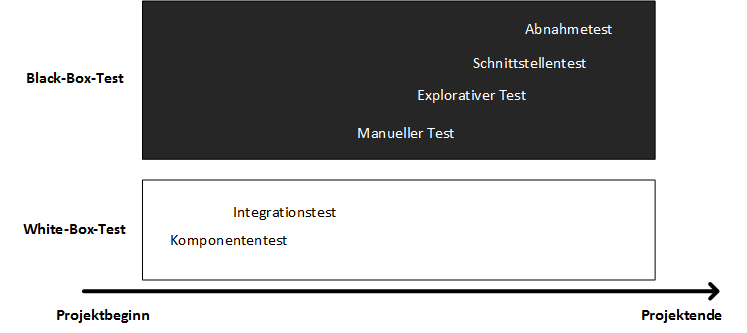
\includegraphics[width=0.9\textwidth]{testuebersicht.png}
\caption{Testmethoden unterteilt in \enword{White-Box-} und \enword{Black-Box}-Testen}
\label{fig:testtypen}
\end{figure}

\SuperPar
Funktionale Tests haben die Aufgabe sicherzustellen, dass die Anforderungen aus der Spezifikation korrekt umgesetzt werden. Für die Umsetzung dieser Tests können sowohl manuelle als auch automatisierte Testmethoden verwendet werden, welche in Abbildung \ref{fig:testtypen} dargestellt sind. Die unterschiedlichen Methoden werden in diesem Kapitel genauer beschrieben und es wird auf die Unterschiede eingegangen.

\SuperPar
Im zweiten Teil dieses Kapitels werden die verwendeten Technologien beschrieben. Dazu gehören die Werkzeuge und Bibliotheken, welche für die Entwicklung von Rayden verwendet werden. Diese Werkzeuge und Bibliotheken werden benötigt, da Rayden aus einer Sprache, einem Compiler, einem Interpretierer und weiteren Komponenten besteht. Weiters werden zwei Testtreiber-Bibliotheken beschrieben, welche für automatisierte Abnahmetests verwendet werden können. 

\section{\enword{White-Box}-Test}

Unter \enword{White-Box}-Tests versteht man Tests, bei denen die Testerinnen und Tester Zugriff auf den Quelltext haben. \enword{White-Box}-Tests werden speziell für bestimmte Codefragmente geschrieben und testen gezielt einzelne Teile einer Anwendung. Diese Tests werden in einer frühen Phase des Entwicklungsprozesses erstellt und liefern sehr bald Qualitätskennzahlen. 

\SuperPar
\enword{White-Box}-Tests sind typischerweise sehr technisch und verlangen vom Testpersonal Programmierkenntnisse. Daher werden diese Tests von Personen aus der Entwicklungsabteilung selbst geschrieben und fallen nicht in den Zuständigkeitsbereich des Qualitätssicherungsteams. Das gilt natürlich nur solange, als man sich nicht in einem agilen Entwicklungsprozess befindet. Dort werden sowohl die \enword{White-Box}- als auch die \enword{Black-Box}-Tests im Entwicklungsteam umgesetzt.


\section{\enword{Black-Box}-Test}

Die \enword{Black-Box}-Tests sind klassische Aufgaben eines Qualitätssicherungsteams. Sie umfassen alle Testansätze, bei denen der Quelltext der Anwendung nicht vorliegt. Dabei ist die Anwendung also eine \enword{Black Box}. Die Aufgabe des Qualitätssicherungsteams ist es, zu überprüfen, ob alle Anforderungen laut Spezifikation umgesetzt wurden. Für diese Aufgabe steht dem Qualitätssicherungsteam eine ganze Reihe an unterschiedlichen Ansätzen zur Verfügung, angefangen von manuellen Tests über explorative Tests bis hin zu automatisierten Abnahmetests. 

\SuperPar
Die \enword{Black-Box}-Tests werden typischerweise im fortgeschritten Projektstadium durchgeführt. Das ergibt sich aus der Tatsache, dass man für die \enword{Black-Box}-Tests eine lauffähige Anwendung benötigt.

\section{Manuelle Testmethoden}

Bei manuellen Tests handelt es sich generell um \enword{Black-Box}-Tests. Dabei überprüft die Testerin oder der Tester, ob sich die Anwendung in Bezug auf die in der Spezifikation angegebenen Anforderungen korrekt verhält und ob die Funktionalität vollständig vorhanden ist. Die Funktionalität wird typischerweise über die Benutzeroberfläche geprüft. Eine zusätzliche Aufgabe bei manuellen Tests ist es, zu überprüfen, ob die Benutzeroberflächen-Konzepte korrekt und einheitlich umgesetzt wurden.

\SuperPar
Bei manuellen Tests ist es typisch, dass die Testmanagerin oder der Testmanager eine textuelle Beschreibung der Testfälle erstellt. Diese Testfälle werden dann von dem Qualitätssicherungsteam für jede neue Version der Anwendung durchgeführt. Bei einer Abweichung der Anwendung muss entschieden werden, ob sich der Anwendungsfall geändert hat oder ob die Anwendung nicht korrekt funktioniert. Im letzteren Fall muss ein Fehlerbericht verfasst und an die Entwicklungsabteilung gesendet werden.

%%\subsection{Explorativer Test}

\SuperPar
Eine Spezialform des manuellen Testens ist das explorative Testen. Dabei bekommt die Testerin oder der Tester keine genaue Vorgabe, wie ein Anwendungsfall getestet werden soll. In diesem Fall bekommt die Person nur eine Aufgabe gestellt, welche mit der Anwendung gelöst werden muss. Das Ziel ist es, dass man unterschiedlichste Möglichkeiten der Anwendung testen kann. Dieser Ansatz ist gut dafür geeignet, um neue Fehler zu finden. 

\SuperPar
Grundsätzlich haben manuelle und automatisierte Tests die Limitierung, dass nur festgestellt werden kann, ob eine neue Version einer Anwendung gleich gut funktioniert wie die alte. Es können aber keine neuen Fehler abseits der definierten Tests gefunden werden. Diese Lücke versucht das explorative Testen zu schließen. Es ist auch von Vorteil, wenn nicht immer die gleiche Person dieselbe Aufgabe testet. Jede Person hat neue Ideen, wie man die Aufgabe lösen kann und testet daher neue Bereiche und Kombinationen der Anwendung. Dieser Ansatz ist ein kreativer Prozess und kann daher im Gegensatz zu klassischen manuellen Tests nicht automatisiert werden.

\section{Automatisierte Testmethoden}

Das Ziel von automatisierten Tests ist es, dass man den Testaufwand in einem Softwareprojekt reduziert. Aus wirtschaftlicher Sicht ist es viel besser, wenn das stupide Testen durch einen automatisierten Test erledigt wird. Dadurch reduzieren sich die Kosten für das Softwareprojekt. Bei einer manuellen Ausführung kann es bei mehrmaligen Wiederholungen eines Tests zu Aufmerksamkeitsverlusten kommen, was bei automatisierten Tests nicht der Fall ist.

\SuperPar
Durch automatisierte Tests werden Qualitätssicherungsteams jedoch nicht obsolet. Auf der einen Seite müssen die automatisierten Tests auch von jemandem geschrieben und gewartet werden, auf der anderen Seite sind automatisierte Tests für exploratives Testen ungeeignet. Die Aufgabe des explorativen Testens wird auf absehbare Zeit immer durch Personen erledigt werden.

\SuperPar
Schlussendlich gibt es noch einen weiteren wichtigen Vorteil von automatisierten Tests gegenüber manuellen Tests: Man kann automatisierte Tests viel öfter ausführen und sie liefern schneller eine Aussage über die Qualität der Software. Diese Zeitreduktion ist für agile Softwareentwicklungsprozesse sehr wichtig, denn damit bekommt das Entwicklungsteam schneller eine Rückmeldung darüber, ob das System (noch) korrekt funktioniert. 


\subsection{Komponententest (\enword{Unit Testing})}

Bei einem Komponententest \cite{xUnit} wird genau eine Softwarekomponente getestet. Eine Softwarekomponente ist eine abgeschlossene Einheit in einem Softwareprojekt, welche eine definierte Schnittstelle hat. Das kann zum Beispiel eine einzelne Klasse, aber auch ein ganzes Modul sein, wie zum Beispiel in Pascal. Aus diesem Grund wird der Komponententest auch oft als Modul-Test oder Unit-Test bezeichnet. In dem Fall, dass die zu testende Komponente eine Abhängigkeit von einer anderen Komponente hat, werden diese durch eine Test-Implementierung ersetzt. Der Vorteil von Komponententests ist, dass deren Erstellung und Wartung keinen großen Aufwand verursachen. Das ist auch der Grund, warum dieser Testansatz sehr beliebt und weit verbreitet ist. Die Beliebtheit dieser Variante kann man daran ablesen, dass es mittlerweile für so gut wie jede Programmiersprache eine Unit-Test-Bibliothek wie zum Beispiel \enword{JUnit} \cite{JUnit} gibt. Der Vorteil ist aber auch der größte Nachteil bei diesem Ansatz: Die Komponenten werden einzeln getestet und man kann daher keine Aussage darüber treffen, wie sich das Gesamtsystem verhalten wird.

\SuperPar
Um eine Aussage über das Verhalten des Gesamtsystems zu erhalten, kann man Integrationstests verwenden. Diese werden im nächsten Abschnitt erklärt.

\subsection{Integrationstest (\enword{Integration Testing})}

Der Integrationstest ist schon deutlich aufwendiger und umfangreicher als ein Komponententest. Bei einem Integrationstest werden alle Komponenten eines Softwaresystems gemeinsam getestet. Das Ziel bei diesen Tests ist es zu gewährleisten, dass alle Komponenten miteinander funktionieren und dass alle Schnittstellen korrekt implementiert wurden. Es werden auch unterschiedliche Fehlersituationen im System simuliert und überprüft, ob diese ausgeglichen werden können. Ein einzelner Fehler in einer Komponente soll nicht das ganze System zum Absturz bringen oder in einen ungültigen Zustand versetzen.

\SuperPar
Bei einem Integrationstest stellt sich oft die Frage, ob man mit oder ohne Datenbank testen soll. Diese Frage kann man nicht so einfach beantworten. Auf der einen Seite kann man sagen, dass die Datenbank genauso eine Komponente im Softwaresystem ist, welche getestet werden muss. Auf der anderen Seite kann man argumentieren, dass die Datenbank ein externes System ist, welches bereits getestet wurde. Grundsätzlich ist jedoch zu sagen, dass es ein guter Ansatz ist, wenn man die Integrationstests mit einer Datenbank durchführt. Eine ausführliche Diskussion über diese Thematik kann man in \enword{Der Integrationstest} \cite{intTest} nachlesen. Es kann immer wieder vorkommen, dass genau bei der Schnittstelle zwischen Softwaresystem und Datenbank Probleme auftreten. Diese Fehler würden sonst erst relativ spät im Projekt-Lebenszyklus auftreten und der Aufwand für die Behebung dieser Fehler würde steigen.

\SuperPar
Der Grund, warum über dieses Thema so viel diskutiert wird ist, dass der Aufwand für einen Integrationstest mit Datenbank deutlich höher ist. Man muss eine Strategie finden, wie man für jede Testausführung einen definierten Datenbankzustand herstellen kann. Dieser Datenbankzustand ist sehr wichtig, um reproduzierbare Tests schreiben zu können. 


\subsection{Schnittstellentest (\enword{API Testing})}

Der Schnittstellentest ist die Vorstufe zum Abnahmetest, bei welcher alle externen Schnittstellen getestet werden. Dabei kann es sich um eine Schnittstelle zu einem externen System handeln oder um eine Web-Service-Schnittstelle. Aber darunter fällt auch die Schnittstelle zwischen Benutzeroberfläche und Geschäftslogik. Gerade diese Schnittstelle ist für die Testautomatisierung sehr interessant, da man hierbei die Benutzeroberfläche nicht für das Testen benötigt, jedoch das Gesamtsystem testen kann. Der Vorteil liegt darin, dass dieser Testansatz deutlich stabiler ist als ein Abnahmetest, welcher die Tests über die Benutzeroberfläche ausführt. Auch ist die Durchlaufzeit eines Schnittstellentests deutlich geringer als die eines Abnahmetests.

\SuperPar
Der Unterschied zwischen einem Schnittstellentest und einem Integrationstest ist, dass bei einem Schnittstellentest das Software-System vollständig installiert wird. Für die Tests wird eine vollwertige Datenbank mit realistischen Testdaten verwendet. Bei einem Integrationstest verzichtet man auf diesen Aufwand.

\SuperPar
Wie schon die vorhergehenden Testansätze hat auch dieser Ansatz einen großen Nachteil: Bei diesen Tests werden nur die Schnittstellen zwischen externem System und der Benutzeroberfläche getestet. Dabei kann aber nicht sichergestellt werden, dass die Benutzeroberfläche fehlerfrei funktioniert. Für die Benutzerin oder den Benutzer der Anwendung zählt aber schlussendlich nur, ob die Verwendung über die Benutzeroberfläche korrekt funktioniert. Aus diesem Grund sind all diese Testansätze kein Ersatz für die Abnahmetests.

\subsection{Abnahmetest (\enword{User Acceptance Testing})}

Abnahmetests sind die aufwendigsten und kostenintensivsten Aufgaben im Testprozess. Bei einem Abnahmetest wird die Anwendung aus Sicht der Benutzerin oder des Benutzers getestet. Das Qualitätssicherungsteam verifiziert, ob alle Anwendungsfälle und Funktionen, welche in der Spezifikation definiert worden sind, vorhanden sind. Dafür muss eine lauffähige Anwendung vorhanden sein, um diese Tests durchführen zu können. Im Wasserfall-Vorgehensmodell kommt dieser Testansatz am Ende des Entwicklungszyklus. Es kommt dabei nicht selten vor, dass die Kundin oder der Kunde diese Tests manuell durchführt. Bei den agilen Vorgehensmodellen werden diese Tests nach jeder Iteration durchgeführt. Durch die kurzen Iterationszyklen können die Abnahmetests nicht mehr manuell durchgeführt werden. In diesem Fall kommen automatisierte Abnahmetests zum Einsatz. 

\SuperPar
Die große Herausforderung bei diesem Testansatz ist es, die Balance zwischen manuellen und automatisierten Tests zu finden.

\section{Verwendete Technologien}

Rayden basiert auf und verwendet eine Vielzahl von unterschiedlichen Technologien, Werkzeugen und Bibliotheken. Dieser Abschnitt gibt einen Einblick in diese Technologien und erklärt, in welchen Bereichen diese im Rayden-System verwendet werden. Als Basis wird die Programmiersprache Java und deren Laufzeitumgebung verwendet. Die Entscheidung für Java ist essentiell für das Projekt, um eine große Anzahl an unterschiedlichen Test-Szenarien zu unterstützen. 

\SuperPar
Für die Umsetzung der Sprache Rayden wurden viele Bibliotheken und Werkzeuge aus dem Eclipse-Umfeld verwendet. Als Testtreiber-Bibliotheken werden sowohl die offene Selenium- als auch die kommerzielle \enword{Borland Silk Test}-Implementierung verwendet.

\subsection{Eclipse}

Eclipse \cite{Eclipse} ist eine Entwicklungsumgebung für eine Vielzahl an Programmiersprachen. Ursprünglich wurde Eclipse von IBM für die Sprache Java entwickelt. Im Laufe der Zeit wurde Eclipse zu einer beliebten Entwicklerplattform und es wurden immer mehr Sprachen über \enword{Plug-ins} unterstützt. Auch für das Rayden-System soll ein solches \enword{Plug-in} entwickelt werden, um eine gute Unterstützung bei der Erstellung von Tests bieten zu können. 

\SuperPar
Neben der Entwicklungsumgebung ist Eclipse aber auch eine Plattform für die unterschiedlichsten Projekte geworden. Diese Projekte werden von der \enword{Eclipse Foundation} \cite{EclipseFoundation} verwaltet und durch Partnerunternehmen und Freiwillige gepflegt. 

\SuperPar
Einige dieser Projekte werden in den nächsten Abschnitten separat vorgestellt.

\subsection{\enword{Eclipse Modeling Framework}}

Das \enword{Eclipse Modeling Framework} (EMF) \cite{EMF} ist ein Modellierungswerkzeug für Java. EMF stellte eine Menge an Werkzeugen zur Erstellung, Verwaltung und Weiterverarbeitung zur Verfügung. Dazu gehört auch die Möglichkeit, aus diesen Modellen Code zu generieren. Eine Kernkomponente von EMF ist das \enword{ECore}-Metamodell. Ein Metamodell ist die Schablone für ein spezifisches Modell. Aus einem \enword{ECore}-Modell kann man mithilfe von Code-Generatoren eine Java-Bibliothek generieren.

\SuperPar
Auf diesem Konzept baut auch das xText-Projekt auf, welches im nächsten Abschnitt vorgestellt wird. 

\subsection{xText}

Das xText-Projekt \cite{xtext} unterstützt das Erstellen von neuen Sprachen. Grundsätzlich ist xText ein Compiler-Generator der aus einer Grammatik einen lexikalischen und einen Syntax-Analysator generiert. Das Besondere an xText ist aber, dass man noch zusätzlich einen Eclipse-Editor für die Sprache bekommt. Der Editor bietet grundlegende Funktionen wie Syntax-\enword{Highlighting}, Fehler- und Validierungsmechanismen. Diese Funktionalität kann man nachträglich noch anpassen und weitere Funktionen hinzufügen. Ein Vorteil von xText ist, dass man den generierten Compiler auch außerhalb von Eclipse als eigenständige Anwendung verwenden kann. Somit kann der Aufwand, zwei Compiler für seine Sprache warten zu müssen, eingespart werden. Der abstrakte Syntaxbaum einer Quelldatei wird im Compiler mit EMF umgesetzt. Das heißt, man bekommt einen vollständigen Syntax-Baum im Hauptspeicher, welchen man sehr einfach verarbeiten kann. Um die Verwendung noch zu vereinfachen, liegt für den Baum ein Metamodell in Form eines \enword{ECore}-Modells vor. 

\subsection{Selenium}

Selenium \cite{Selenium} ist eine Open-Source-Bibliothek, um Web-Seiten automatisiert testen zu können. Die Bibliothek unterstützt eine Vielzahl an unterschiedlichen Browsern auf allen gängigen Betriebssystemen wie Windows, Linux, Macintosh und Google Android. Um die Browser ansprechen zu können, benötigt man einen speziellen Treiber. Dieser wird entweder als separate Anwendung aus- oder bereits mit dem Browser mitgeliefert.

\SuperPar
In der ersten Version hat Selenium auf eine proprietäre Programmierschnittstelle gesetzt. Seit der Version 2 setzt Selenium auf die standardisierte Programmierschnittstelle \enword{WebDriver} \cite{WebDriver} des W3C Konsortiums. Der Vorteil von \enword{WebDriver} ist, dass man eine einheitliche Programmierschnittstelle für die unterschiedlichsten Browser hat. Damit erzielt man Unabhängigkeit von einem spezifischen Browser. 

\subsection{Borland Silk Test}

\enword{Borland Silk Test} \cite{SilkTest} ist eine kommerzielle Testsoftware für native wie auch Web-Anwendungen. \enword{Borland Silk Test} bietet Unterstützung für eine Vielzahl an unterschiedlichen Technologien. Unterstützt werden zum Beispiel die gängigen Browser wie Internet Explorer, Google Chrome und Mozilla Firefox. Neben Web-Technologien werden auch native Windows-, Adobe-Flex-, Windows-Presentation-Foundation- oder Java-Anwendungen unterstützt. Seit kurzem werden auch Browser und Anwendungen  auf mobilen Geräten unterstützt. Der Vorteil von \enword{Silk Test} gegenüber von Selenium ist, dass es einen verbesserten \enword{X-Browser Support} gibt. Dabei kann man einen Test, welchen man zum Beispiel mit dem Internet Explorer aufzeichnet, mit einem Mozilla-Firefox- oder dem Google-Chrome-Browser ausführen. Durch diese \enword{X-Browser}-Technologie entfällt die Wartung von Tests für die verschiedenen Browser. 

\chapter{Aufbau und Ablauf von Testprojekten}
\label{cha:Konzept}

Diese Kapitel befasst sich mit den Testabläufen in einem Softwareprojekt. Diese Abläufe finden in unterschiedlichen Phasen eines Softwareprojekts statt und werden von unterschiedlichen Personengruppen durchgeführt. Diese Kapitel gibt einen Einblick in diese Abläufe und beschreibt auch die Schwierigkeiten, die es in einem Testprojekt zu bewältigen gibt. Im zweiten Abschnitt wird die Evolution der Testautomatisierung beschrieben. Dabei werden unterschiedliche Testansätze vorgestellt, welche sich über die Zeit entwickelt haben. Einer diese Testansätze stellt die Basis für das Rayden-System dar.

\section{Ablauf eines Testprojekts}

In einem Softwareentwicklungsprojekt gibt es nicht nur die Test-Phase, in welcher die Testabteilung eine wichtige Rolle spielt. Die Testabteilung ist in den meisten Phasen eines Entwicklungsprojekts involviert. Um die gesamten Testaufgaben in einem großen Projekt zu koordinieren, wir oft ein Testprojekt aufgesetzt. In einem Testprojekt werden alle Aktivitäten rund um die Qualitätssicherung vereint. Diese Aktivitäten beschränken sich aber nicht nur auf die Testabteilung. Es müssen auch Personen aus der Fachabteilung und der Entwicklungsabteilung eingebunden werden. Diese Schnittstellen zwischen den einzelnen Abteilungen bieten eine große Herausforderung für die Testmanagerin oder dem Testmanager.

\SuperPar
In den nachfolgenden 6 Abschnitten werden die einzelnen Aufgaben in eine Testprojekt beschrieben. Es wird beschrieben, wie Testfälle entwickelt werden und zu welchem Zeitpunkt in einem Softwareprojekt welche Testaktivitäten ablaufen.

\subsection{Rollen in einem Testprojekt}

Das Testprojekt besteht aus einer bunten Mischung an unterschiedlichen Personen. Die Verantwortung in einem Testprojekts trägt die Testmanagerin oder der Testmanager. Diese Person ist für die Koordination des Projekts zuständig und bildet die Schnittstellen zu anderen Abteilungen. Eine Schnittstellen besteht zu der Fachabteilung. Von der Fachabteilung werden die Anwendungsfälle geliefert welche in weiterer Folge in der Testabteilung umgesetzt werden. Für die Umsetzung der Testfälle sind die Testerinnen und die Tester zuständig. Für die Automatisierung von Testfällen besteht eine Schnittstelle zu der Entwicklungsabteilung, falls die Testabteilung über keine eigene Entwicklerinnen oder Entwickler verfügt.

\subsection{Testfall}

Während der Konzeptionsphase in einem Entwicklungsprojekts werden Anforderungen von der Fachabteilung aufgenommen. Aus diesen Anforderungen werden Anwendungsfälle abgeleitet. Auf Basis dieser Anwendungsfälle werden in der Testabteilung Testfälle von den Testerinnen und Testern abgeleitet.

\todo

\subsection{Komponenten- und Integrationstests für Testfälle}

TODO !!!

\subsection{Manuelle Abnahmetests für Testfälle}

TODO !!!

\subsection{Automatisieren von manuellen Abnahmetests}

TODO !!!

\subsection{Testdokumentation}

TODO !!!

\section{Evolution der Testautomatisierung}

Die Automatisierung von Abnahmetests hat sich über die Zeit einen starken Wandel unterzogen. In diesem Bereich hat es eine ähnliche starke Entwicklung wie bei den Softwareentwicklungstechniken gegeben. Im Jahr 2009 haben Jeff Hinz und Martin Gijsen eine Artikel \cite{Hinz09} über die Evolution der Testautomatisierung veröffentlicht. In diesem Artikel teilen die beiden Autoren die Entwicklung der Testautomatisierung in fünf Generationen ein. Jede Generation zeichnet sich durch eine spezielle Technik aus, wie die Test entwickelt werden. 

\begin{figure}
\centering
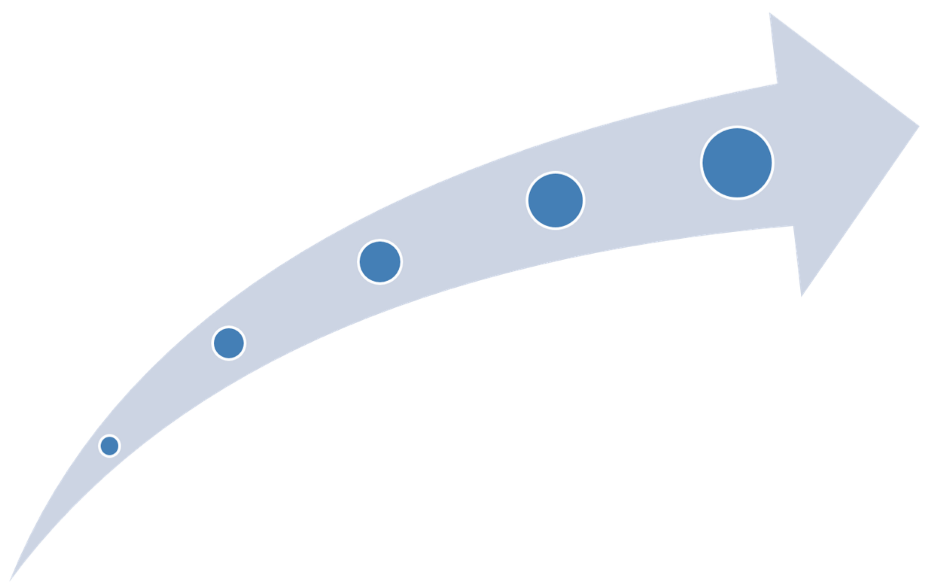
\includegraphics[width=0.9\textwidth]{EvolutionVonTest.png}
\caption{Die fünf Generationen von Testtechniken}
\label{fig:testEvolution}
\end{figure}

\SuperPar
Die Abbildung \ref{fig:testEvolution} zeigt die einzelnen Entwicklungsstufen. In den nächsten Abschnitten werden die Techniken vorgestellt und auf die Vorteile und Nachteile eingegangen.

\subsection{Erste Generation - \enword{Record-Replay}}

Die erste Generation von Testtechniken sind die \enword{Record-Replay}-Ansätze. Dieser Ansatz besteht aus zwei Phasen. In der ersten Phase wird mithilfe einer Analyse-Software die Aktionen der Benutzerin oder des Benutzers mit der Anwendung aufzeichnet. Dabei werden typischerweise die Mausbewegungen und die Tastatureingaben aufgezeichnet. In der zweiten Phase werden die aufgezeichneten Aktionen mit einer speziellen Software wieder abgespielt. Die Testsoftware beinhaltet dazu spezielle Maus- und Tastatur-Treiber, um die aufgezeichneten Aktionen wiedergeben zu können.

\SuperPar
Der große Vorteil bei dieser Methode ist die Einfachheit. Zum Aufzeichnen von Tests muss die Testerin oder der Tester den Anwendungsfall durcharbeiten und im Hintergrund werden die Aktionen aufgezeichnet. Für diese Testtechnik werden keine speziellen Fähigkeiten benötigt. Jedoch hat diese Technik einen massiven Nachteil. Sobald sich die zu testende Anwendung nur marginal an der Oberfläche ändert, funktioniert diese Testmethode nicht mehr. Auch müssen die Tests immer mit der selben Bildschirmauflösung ausgeführt werden, um die Aktionen korrekt wiedergeben zu können. Ein weiterer Nachteil ist, dass sobald man einen Test ändern möchte, muss man den gesamten Test neu aufzeichnen.

\subsection{Zweite Generation - \enword{Functional Decomposition}}

Bei \enword{Functional Decomposition} werden die Tests in einzelne Testsequenzen zerteilt. Mit dieser Technik konnten langen unleserliche Test in handliche Sequenzen zerteilt werden. Die Methode erlaubt auch die Wiederverwendung von Sequenzen in anderen Tests. Durch einen hohen Wiederverwendungsgrad kann die Größe des Testprojekts stark reduziert werden. Ein weiterer positive Effekt kann man in der Wartbarkeit des Testprojekts feststellen. Durch die Reduktion der Test wird auch der der Wartungsaufwand geringer.

\SuperPar
Mit dieser Testmethode war es nun auch möglich, Bibliotheken mit Testfunktionen für ein Testprojekt anzulegen. 

\subsection{Dritte Generation - \enword{Data-Driven Testing}}

In der dritten Generation von Testmethoden wurde ein großes Augenmerk auf die Testdaten gelegt. In den vorgehenden Testtechniken lag der Fokus auf der Erstellung und Wartung von Testprojekten. Dabei mussten auch schon Testdaten verwendet werden, aber der Stellenwert war nicht hoch. Die Testdaten stehen dafür nun in dieser Generation im Mittelpunkt. Man erkannte, dass man oft die selbe Testsequenz durchläuft, aber jedes Mal andere Daten verwendet. Diese Testtechnik wird stark für datenzentrierten Anwendungen verwenden. 

\SuperPar
Bei einem \enword{Data-Driven-Testing} werden im Test keine konkrete Werte verwendend. Statt dessen werden Platzhalter (Variablen) im Test eingebaut. Bei der Ausführung eines Tests werden die Platzhalter mit einem Wert aus einer Datenquelle verbunden. Als Datenquelle können Dateien wie auch Datenbanken dienen. Mit dieser Technik, kann man ein und denselben Test mit unterschiedlichen Daten ausführen. 

\subsection{Vierte Generation - \enword{Keyword-Driven Testing}}

In der vierten Generation von Testmethoden werden die Testdaten noch weiter in den Mittelpunkt gestellt. Bis zu diesem Zeitpunkt wurden die Test entweder mithilfe eines \enword{Record-Replay}-Ansatzes aufgezeichnet oder in einer Programmiersprache entwickelt. Der \enword{Record-Replay}-Ansatz war einfach und auch von nicht technisch versierten Personen zu benutzen. Jedoch haben diese aufgezeichneten Test ein Zuverlässlichkeitsproblem. Der zweite Ansatz bedingt, dass die Personen aus der Testabteilung Programmierkenntnisse benötigen.

\SuperPar
Bei \enword{Keyword-Driven-Testing} wurden die Tests nun auch als Testdaten angesehen. Mit diesem Ansatz können Tests mit dem gleichen Ansatz wie die Testdaten erstellt und verwaltet werden. Um einen \enword{Keyword-Driven}-Test ausführen zu können, wird ein spezieller Interpreter benötigt. Der Interpreter liest die Tests über eine Datenquelle ein und arbeitet diese ab. Für die Verarbeitung müssen die Tests in einem lesbaren Format für den Interpreter vorliegen. Eine detaillierte Beschreibung liefert Pekka Laukkanen von der Universität von Helsinki in seiner Masterarbeit \cite{Lauk06}. 

\subsection{Fünfte Generation - \enword{Scriptless Automation}}

Die letzte Methode versucht die Testautomatisierung mit einem \enword{Scriptless-Automation}-Ansatz zu vereinfachen. Bei diesem Ansatz wird versucht, dass man aus einer abstrakten Repräsentation eines Tests den Code zu erzeugen. Bei diesem Transformationsvorgang werden Code-Vorlagen und Code-Generatoren verwendet.

\SuperPar
Bei diesem Ansatz wird wiederum versucht, die Größe des Testprojekts zu reduzieren und somit die Wartbarkeit zu erhöhen. Diese Ansatz befindet noch in einer frühen Phase und hat in der Praxis bis jetzt noch keine Relevanz. 

\SuperPar
Im nächsten Abschnitt wird eine Implementierung des \enword{Keyword-Driven-Testing} vorgestellt, welches die Grundlage für das Rayden-System ist.

\section{\enword{Robot-Framework}}

Das \enword{Robot-Framework} \cite{Robot} ist die Umsetzung des \enword{Keyword-Driven-Testing}-Ansatzes und wurde ursprünglich von Nokia Siemens Networks entwickelt. Später wurde das Projekt unter die Apache 2 Lizenz gestellt und veröffentlicht. Das \enword{Robot-Framwork} stellt nicht nur eine technische Basis zur Verfügung, sondern bietet auch ein Vorgehensmodell dafür an. Das Vorgehensmodell wird \enword{Acceptance test-Driven Development} (ATDD) genannt und im Artikel \cite{Lar10} erklärt.

\begin{program}
\begin{JavaCode}
*** Test Cases ***
Anmelden an der PetClinic Anwendung
	[Documentation]	Man meldet sich bei der Anwendung PetClinic mit 
	...             den definierten Daten an. Wenn das Keyword 
	...             erfolgreich ausgeführt worden ist, befindet man 
	...             sich auf der Hauptseite der Webanwendung.
	
	Open Browser	${URL}		${Browser}
	Input Text    user			TestUser
	Input Text		password	secret
	Click Button	login

\end{JavaCode}
\caption{Beispiel von einem \enword{Robot-Framework}-Testfall}
\label{prog:robotTestCase}
\end{program}

\SuperPar
Das \enword{Robot-Framework} verwendet als Testdaten-Format eine Tabulator-Syntax. Dabei werden die Daten durch Tabulatoren getrennt. Die Abbildung \ref{prog:robotTestCase} zeigt einen Testfall, welcher in der Tabulator-Syntax definiert worden ist. In dem Testfall wurde die Selenium-Bibliothek für das \enword{Robot-Framework} verwendet. 

\SuperPar
Das \enword{Robot-Framework} unterstützt die Verwendung von Bibliotheken. In einer Bibliothek können \enword{Keywords} zusammengefasst werden. Das \enword{Robot-Framework} und die Entwickler dahinter stellen eine große Anzahl an vorgefertigten Bibliotheken zur Verfügung. Die vorgefertigten Bibliotheken erleichtern und beschleunigen das Entwickeln von Test enorm. Somit muss man nicht bei jedem neuen Projekt von Null beginnen, sonder kann auf einen Fundus an \enword{Keywords} zurück greifen.

\SuperPar
Ein anderer Vorteil dieser Bibliotheken ist es, dass auch Person ohne technischem Hintergrund dieses \enword{Robot-Framework} verwenden können. Die Bibliotheken sind weitestgehend vollständig, dass man nur selten in die Lage kommt, in der man neue \enword{Keywords} implementieren muss.

\SuperPar
Neben den vielen Vorteil des \enword{Robot-Framework}, gibt es aber auch Nachteile. Ein Nachteil wäre die Tabulator-Syntax. Diese Syntax ist Fehleranfällig und ohne einem speziellen Editor nur mühsam zum lesen. Auch fügt sich die Unterstützung von Kontrollstrukturen nicht optimal in das System ein.

\SuperPar
Das \enword{Robot-Framework} und die identifizierten Probleme bilden den Startpunkt für das Rayden-System, welches im nächsten Kapitel beschrieben wird.


\chapter{Design von Rayden}
\label{cha:Design}

Im vorigen Kapitel wurde der Ablauf eines Testprojekts aufgezeigt und eine Einführung in das Thema \enword{Keyword-Driven Testing} gegeben. In diesem Kapitel wird das Rayden-System detailliert erklärt. Zu Beginn werden die Designziele der Sprache Rayden erklärt. Die Sprache Rayden ist eine domänenspezifische Sprache, welche einige Eigenheiten und Überraschungen enthält. In den weiteren Abschnitten wird der Aufbau des Rayden-Systems erklärt und auf die technischen Details eingegangen. Am Ende dieses Kapitels wird noch die Integration in die \enword{Java-Scripting-API} \cite{JavaScriptApi} beschrieben. Das Rayden-System bietet die Möglichkeit, dass man einen Test in einer Java-Anwendung über das \enword{Java-Scripting-API} ausführen kann.

%%------------------------------------------------------------------------------------------------------

\section{Designziele von Rayden}

Das primäre Designziel von Rayden ist Offenheit. Rayden soll im gesamten Testprozess einsetzbar sein, darf aber die involvierten Personen nicht überfordern. Um dieses Ziel zu erreichen, setzt das Rayden-System auf mehreren Ebenen an.

\SuperPar
Die domänenspezifische Sprache von Rayden ist speziell für Personen im Testbereich ausgelegt. Das wichtigste Ziel der Sprache ist Einfachheit. Die Sprache soll Personen ohne Programmierkenntnisse in die Lage versetzen, Tests in dieser Sprache zu lesen und zu bearbeiten. Die Sprache Rayden ist daher stark an der natürlichen Sprache angelehnt, um den Einstieg zu erleichtern. Ein anderes Ziel bei dem Sprachdesign ist die Flexibilität der Sprache. Der Testprozess setzt sich aus einer Vielzahl an unterschiedlichen Aufgaben zusammen. Um möglichst alle Aufgaben mit dieser Sprache abdecken zu können, wird eine hohe Flexibilität benötigt. 

\SuperPar
Abgesehen von einer geeigneten Sprache gibt es noch weitere wichtige Ziele für das Rayden-System. Rayden muss plattformunabhängig sein, um viele Anwendungsszenarien abdecken zu können. Aus diesem Grund wird die Programmiersprache \enword{Java} für die Entwicklung des Rayden-Systems gewählt. Der Interpreter für Rayden selbst läuft auch wieder auf der virtuellen \enword{Java}-Maschine (JVM).

\SuperPar
Die Einbindung von externen Test-Treiber-Bibliotheken wird durch eine offene Schnittstelle ermöglicht. Dadurch können mit Rayden-Tests für die unterschiedlichsten Anwendungsszenarien entwickelt werden. Rayden kann somit für das jeweilige Projekt und die beteiligten Personen angepasst werden. 

%%------------------------------------------------------------------------------------------------------

\section{Aufbau des Rayden-Systems}

In diesem Abschnitt wird der Aufbau des Rayden-Systems von zwei Blickwinkeln aus beleuchtet. Zuerst wird der konzeptionelle Aufbau erklärt. Dabei wird darauf eingegangen, wie die einzelnen Konzeptebenen miteinander kommunizieren und welche Person für die jeweilige Ebene verantwortlich ist. Im zweiten Teil wird die technische Architektur des Rayden-Systems erläutert. Dazu werden die Komponenten und ihre Beziehungen überblicksweise erklärt. Eine ausführliche Beschreibung findet man in den Abschnitten \ref{cha:KonzeptAufbau} und \ref{cha:TechArch}.

\subsection{Konzeptioneller Aufbau}
\label{cha:KonzeptAufbau}

Wie schon in vorigen Abschnitten erwähnt, ist Rayden an das Konzept von \enword{Keyword-Driven Testing} angelehnt. Bevor der Aufbau von Rayden beschrieben wird, wird der konzeptionelle Aufbau von \enword{Keyword-Driven Testing} erläutert. 

\begin{figure}[h]
\centering
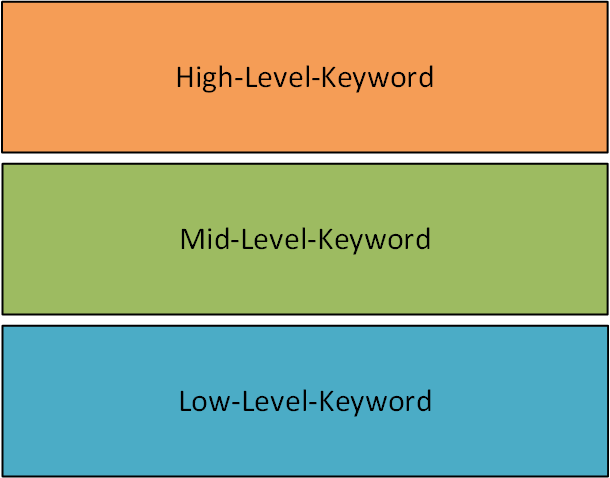
\includegraphics[width=0.7\textwidth]{KDT-Architektur.png}
\caption{Aufbau von \enword{Keyword-Driven Testing}}
\label{fig:kdt-arch}
\end{figure}

\SuperPar
Ein \enword{Keyword-Driven}-Test besteht aus einer Sequenz von \enword{Keywords}. Diese \enword{Keywords} können wiederum aus einer Sequenz von \enword{Keywords} bestehen oder mit einem Codestück verbunden sein. Die \enword{Keywords} werden in drei Kategorien, wie in Abbildung \ref{fig:kdt-arch} dargestellt, aufgeteilt. Die \enword{High-Level Keywords} repräsentieren einen Testfall mit einer detaillierten Beschreibung. Diese Gruppe von \enword{Keywords} wird typischerweise von einer Person aus der Fachabteilung oder von einer Testmanagerin oder einem Testmanager erstellt. Dabei wird aber nur der Rumpf des \enword{Keywords} erstellt. Die Implementierung wird erst in der nächsten Phase hinzugefügt. Diese \enword{High-Level Keywords} bilden die Grundlage für die Erstellung der Tests. In der weiteren Phase werden diese \enword{Keywords} von Testerinnen und Testern implementiert.

\SuperPar
Die \enword{High-Level Keywords} bestehen typischerweise aus einer Sequenz von \enword{Mid-Level Keywords}. Diese Sequenz wird in der zweiten Phase erstellt. Normalerweise finden sich \enword{Mid-Level Keywords} in dieser Sequenz, es können aber auch \enword{Low-Level Keywords} verwendet werden. Die verwendeten \enword{Mid-Level Keywords} bestehen wiederum aus einer Sequenz von \enword{Mid-Level Keywords} und \enword{Low-Level Keywords}. Technisch gesehen gibt es keinen Unterschied zwischen \enword{High-Level Keywords} und \enword{Mid-Level Keywords}. Der Unterschied besteht nur in der Art der Verwendung. \enword{High-Level Keywords} beschreiben genau einen Anwendungsfall der getestet werden soll. Im Gegenteil zu \enword{Mid-Level Keywords} wird hier kein Wert auf Wiederverwendung gelegt.

\SuperPar
In der letzten Phase werden \enword{Low-Level Keywords} mit Code verbunden. Der Code kann prinzipiell in jeder Programmiersprache geschrieben sein. Die Wahl der Programmiersprache hängt von dem verwendeten \enword{Keyword-Driven Framework} ab. In diesen \enword{Keyword-Driven Frameworks} werden häufig Skript-Sprachen verwendet. Der Vorteil von Skript-Sprachen liegt darin, dass der Code für die Ausführung des Tests nicht kompiliert werden muss.

\begin{figure}[h]
\centering
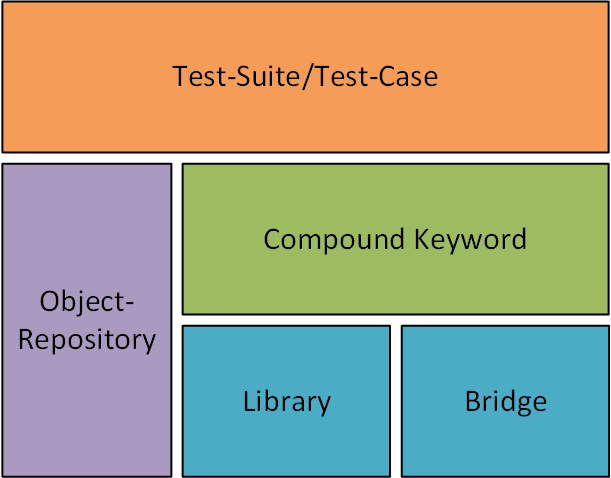
\includegraphics[width=0.7\textwidth]{Rayden-Architektur.png}
\caption{Aufbau von Rayden}
\label{fig:rayden-arch}
\end{figure}

\SuperPar
Im Gegensatz zu \enword{Keyword-Driven Testing} unterteilt das Rayden-System die \enword{Keywords} in mehr Gruppen, wie in Abbildung \ref{fig:rayden-arch} dargestellt. Die zusätzlichen Gruppen bieten einen bessere Strukturierung und geben eine klare Richtung vor, wie ein Rayden-Test-Projekt aufgebaut werden soll.    

\SuperPar
Rayden führt eine klare Trennung bei \enword{Low-Level Keywords} ein. Diese \enword{Keywords}, welche mit einem Codestück verbunden sind, werden in \enword{Library-} und \enword{Bridge-Keywords} unterteilt. \enword{Library-Keywords} stellen grundlegende Funktionen bereit, welche unabhängig von einem speziellen Anwendungsfall sind. Als Beispiel kann man sich eine \enword{For}- oder \enword{Print-Keyword} vorstellen. Im Gegensatz dazu sind \enword{Bridge-Keywords} speziell für eine Anwendungstechnologie angepasst, wie zum Beispiel \enword{Open Browser} oder \enword{Navigate To} für Web-Anwendungen. 

\SuperPar
Auch bei den \enword{High-Level Keywords} bietet Rayden eine größere Vielfalt. Grob werden diese in Test-Suiten und Testfälle unterteilt. Die Test-Suite dient als Gruppierungselement für Testfälle, um diese gemeinsam ausführen zu können. Bei der Definition von Testfällen können diese mit unterschiedlichen Testtypen angelegt werden. Eine nähere Beschreibung findet sich im Abschnitt \ref{cha:KeywordTypes}.

\SuperPar
Zum Abschluss ist noch auf das \enword{Object-Repository} hinzuweisen. Diese Komponente verwaltet Test-Objekte. Test-Objekte können für die Beschreibung von Benutzeroberflächen-Komponenten wie Schaltflächen oder Eingabefelder verwendet werden. Dafür wird für jedes Test-Objekt ein Bezeichner definiert, mit welchem man die Komponente in der Benutzeroberfläche finden kann. Das ist im Fall einer Web-Anwendung ein \enword{XPath}- oder ein \enword{CSS}-Ausdruck. Das \enword{Object-Repository} sorgt somit für eine klare Trennung zwischen Test- und Benutzeroberflächen-Beschreibung. Diese Trennung erhöht die Wiederverwendbarkeit von \enword{Keywords} und reduziert den Wartungsaufwand bei Änderungen an der Benutzerschnittstelle.

\subsection{Technische Architektur}
\label{cha:TechArch}

Die technische Basis für das Rayden-System ist die \enword{Java}-Plattform. Auf der Entwicklungsseite wird \enword{Java} als Programmiersprache für das gesamte Rayden-System verwendet, auf der Ausführungsseite läuft das Rayden-System auf der virtuellen Java-Maschine (JVM). Außerdem bietet Rayden die Möglichkeit, dass man einen Rayden-Test über das \enword{Java Scripting API} \cite{JavaScriptApi} ausführen kann. 

\begin{figure}[h]
\centering
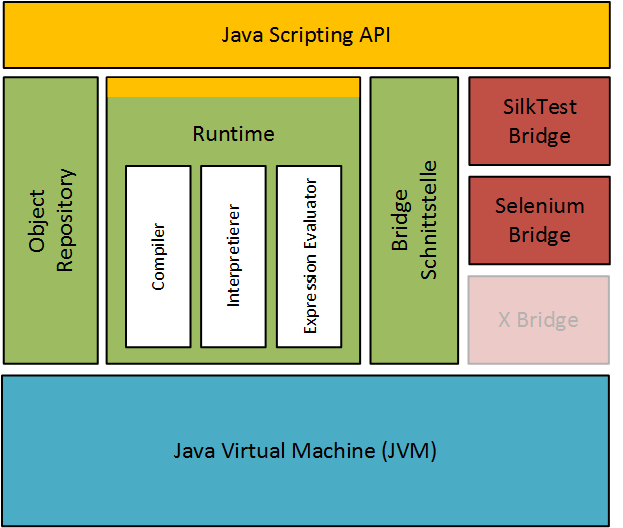
\includegraphics[width=0.9\textwidth]{Rayden-Tech-Architektur.png}
\caption{Rayden-Architektur}
\label{fig:rayden-tech-arch}
\end{figure}

\SuperPar
Abbildung \ref{fig:rayden-tech-arch} zeigt alle Komponenten des Rayden-Kernsystems in Grün. Diese Komponenten bilden die Grundlage dafür, einen Rayden-Test ausführen zu können. Als Basis dieser Komponenten sieht man in Blau die virtuelle Java-Maschine (JVM). Die externen \enword{Bridge}-Implementierungen werden in Rot dargestellt. Diese Komponenten stellen eine Verbindung zwischen dem Test-Treiber und der Rayden-\enword{Runtime} her und werden über die \enword{Bridge}-Schnittstelle hergestellt. Im oberem Abschnitt der Abbildung \ref{fig:rayden-tech-arch} sieht man das \enword{Java Scripting API}, über welches man Rayden-Tests ausführen kann.

\SuperPar
Im nächsten Absatz werden die einzelnen Komponenten der Rayden-Architektur beschrieben, um einen groben Überblick über die Funktionsweise von Rayden zu geben.\\

\begin{itemize}

\item \textbf{Runtime}

Die \enword{Runtime} ist der Einstiegspunkt für die Ausführung von Rayden-Tests. Dazu enthält diese Komponente die Implementierung für die \enword{Java Scripting API}. Wird ein Test ausgeführt, werden zuerst alle Projektressourcen in der \enword{Runtime} geladen. Das Projektverzeichnis kann man über einen Kontextparameter setzen. Falls dieser nicht gesetzt ist, wird das aktuelle Verzeichnis verwendet. Für das Laden der Ressourcen wird die Compiler-Komponente verwendet. Die \enword{Runtime} baut bei diesem Lesevorgang eine \enword{Lookup}-Tabelle für alle \enword{Keywords} auf. Diese Tabelle wird für einen schnellen Zugriff im Interpreter benötigt. Der Rayden-Test wird mithilfe des Interpreters ausgeführt. Das Ergebnis des Tests wird als Resultat über die \enword{Java Scripting API} zurückgegeben.\\

\item \textbf{Compiler}

Der Compiler für die Rayden-Sprache wird mit dem Compiler-Werkzeug xText \cite{xtext} realisiert. Von dem generierten Compiler wird für die Ausführungseinheit nur der lexikalische und syntaktische Analysator verwendet. Der \enword{Eclipse}-Editor wird für das Rayden-System nicht benötigt. Das Resultat der Compiler-Komponente ist ein EMF-Modell des Tests. Die \enword{Runtime}-Komponente verwaltet die Modelle und stellt diese dem Interpreter bei Bedarf zur Verfügung.\\

\item \textbf{Interpreter}

Der Interpreter ist die wichtigste Komponente im Rayden-System. Der Interpreter ist dafür verantwortlich, dass die Rayden-Tests ausgeführt werden können. Zum Starten des Interpreters wird der Aufruf eines \enword{Test-Keywords} übergeben. Dieses \enword{Keyword} wird auf den leeren \enword{Stack} geladen. Der Test wird mithilfe einer \enword{Stack}-Maschine \cite{StackMachine} abgearbeitet. Bei jedem Aufruf eines \enword{Keywords} wird die \enword{Keyword}-Implementierung auf den \enword{Stack} geladen. Zusätzlich wird für jeden neuen \enword{Keyword}-Aufruf ein neuer Gültigkeitsbereich (\enword{Scope}) angelegt. \\
\\
Der Gültigkeitsbereich ist für die Verwaltung der Parameter und Variablen zuständig. Eine Besonderheit in Rayden ist, dass Gültigkeitsbereiche Zugriff auf andere Gültigkeitsbereiche haben. Eine detaillierte Beschreibung dazu findet sich im Abschnitt \ref{cha:KeywordScope}. Die Auswertung von Ausdrücken wird in einem separaten Teil des Interpreters vorgenommen. Für die Auswertung wird der aktuelle Gültigkeitsbereich und der Ausschnitt aus dem Modell an die Evaluierungskomponente übergeben. Das Ergebnis des Ausdrucks wird wieder auf den \enword{Stack} gelegt. Ruft die \enword{Stack}-Maschine ein \enword{Scripted-Keyword} (Beschreibung in Abschnitt \ref{cha:Keyword}) auf, wird entweder der dazugehörige Code ausgeführt oder es wird der Aufruf an die \enword{Bridge}-Schnittstelle weitergeleitet.\\

\item \textbf{Bridge-Schnittstelle}

Die \enword{Bridge}-Schnittstelle ist für die Anbindung von Test-Treibern verantwortlich. Um einen Test-Treiber verwenden zu können, muss eine Rayden-\enword{Bridge} implementiert werden. Die \enword{Bridge} mit der Schnittstelle bildet die Verbindung zwischen der Rayden-\enword{Runtime} und dem Test-Treiber.\\

\item \textbf{Object-Repository}

Das \enword{Object-Repository} verwaltet Test-Objekte, welche von \enword{Keywords} verwendet werden können. Die Test-Objekte werden in einer Baumstruktur verwaltet. Die wichtigste Eigenschaft eines Test-Objekts ist der Bezeichner (\enword{Locator}). Mit dem Bezeichner kann die Benutzerschnittstellen-Komponente identifiziert werden. Das Konzept ist an der Idee von \enword{Page-Object-Pattern} \cite{PageObject} angelehnt. \\

\end{itemize}


%%------------------------------------------------------------------------------------------------------

\section{Sprache von Rayden}

Als Inspiration und Basis für die Sprache dient das Konzept von \enword{Keyword-Driven Testing}. Das Grundprinzip hinter \enword{Keyword-Driven Testing} ist die Verwendung von \enword{Keywords}. Ein \enword{Keyword} besteht aus einer Sequenz von anderen \enword{Keywords} oder ist mit einem Codestück verbunden. Einen \enword{Keyword-Driven}-Test kann man sich auch als gerichteten Graph vorstellen, in dem die Knoten die \enword{Keywords} repräsentieren und die Kanten die Abhängigkeit zwischen den \enword{Keywords} beschreiben, wie in Abbildung \ref{fig:test-graph} dargestellt.

\begin{figure}[h]
\centering
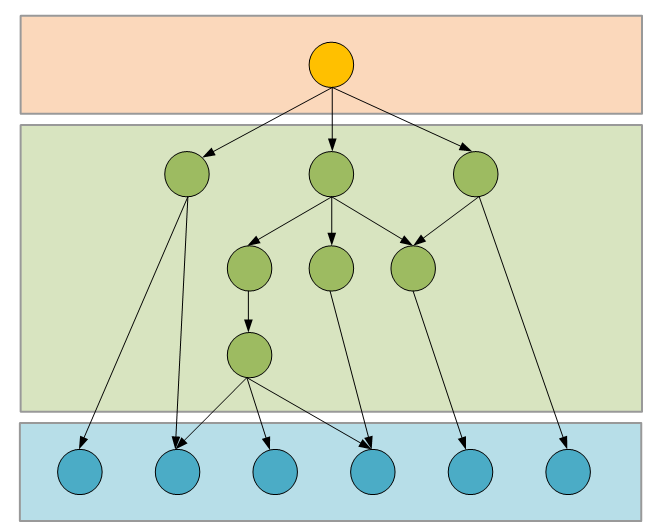
\includegraphics[width=0.8\textwidth]{Rayden-Testbaum.png}
\caption{Graph-Repräsentation eines Tests}
\label{fig:test-graph}
\end{figure}

\SuperPar
Der gelbe Knoten repräsentiert ein \enword{High-Level Keyword}. Von diesem Knoten aus werden über gerichtete Kanten die Beziehungen zu den \enword{Mid-Level Keywords} in Grün definiert. Man sieht, dass die \enword{Mid-Level Keywords} entweder wieder in Beziehungen zu anderen \enword{Mid-Level Keywords} stehen oder \enword{Low-Level Keywords} referenzieren. Die \enword{Low-Level Keywords} werden in Blau dargestellt. Bei den Graphen handelt es um einen gerichteten azyklischen Graph (DAG).

\SuperPar
Die Rayden-Sprache setzt auch auf dieses Konzept von \enword{Keywords}. Im Unterschied zu \enword{Keyword-Driven Testing} setzt Rayden auf eine größere Vielfalt an unterschiedlichen \enword{Keywords}, welche im nächsten Abschnitt \ref{cha:Keyword} detailliert beschrieben werden. Ein weiterer Unterschied ist die Benennung von \enword{Keywords}. Normalerweise besteht der Name eines \enword{Keywords} nur aus einem Wort, damit die Verarbeitung der Tests für den Compiler erleichtert wird. In der Rayden-Sprache wird ein großes Augenmerk darauf gelegt, dass man nicht nur auf ein Wort beschränkt ist, sondern auch ganze Sätze als Namen verwenden kann. Diese Eigenschaft ist sehr nützlich, um die Testfälle wie in einer natürlichen Sprache beschreiben zu können. Der Vorteil ist, dass man somit ohne weiteren Aufwand eine ordentliche Dokumentation des Tests bekommt.

\SuperPar
Eine andere interessante Eigenschaft der Sprache ist, dass in der Sprache keine Sprung-Operationen enthalten sind. Die Konsequenz daraus ist, dass es in der Sprache auch keine Schleifen- oder Verzweigungs-Konstrukte enthalten sind. Die einzige Möglichkeit, um ähnliche Konstrukte zur Verfügung zu stellen, sind \enword{Scripted Compound Keywords}, wobei man bei diesem Metatyp von \enword{Keyword} auch nur entscheiden kann, ob eine Sequenz von \enword{Keywords} ausgeführt werden soll. Das Konzept der Metatypen wird im Abschnitt \ref{cha:Keyword} beschrieben. 

\SuperPar
Da Sprung-Operationen vermieden werden und die Sprache blockstrukturiert ist, gewinnt man die Fähigkeit, Tests visuell darstellen zu können. Diese Fähigkeit ist hilfreich, um eine bessere Unterstützung und einen leichteren Einstieg in die Sprache zu ermöglichen. Das ist vor allem von Vorteil, wenn Personen aus einer Fachabteilung nur unregelmäßig damit arbeiten müssen. 

%%------------------------------------------------------------------------------------------------------

\section{\enword{Keywords} von Rayden}
\label{cha:Keyword}

Das \enword{Keyword} ist die Schlüsselkomponente der Sprache Rayden. In diesem Abschnitt werden die unterschiedlichen Typen und Metatypen erklärt und gezeigt, wofür diese verwendet werden können. Am Anfang werden die vier Metatypen von \enword{Keywords} erklärt. Die Metatypen sind die Basis für den Funktionsumfang der Sprache. Ferner werden die unterstützten Typen beschrieben und wofür diese verwendet werden können. Als Abschluss werden noch Themen wie Sichtbarkeit, Benennung und Parameter erläutert.

%%------------------------------------------------------------------------------------------------------

\subsection{Metatypen}

Der Metatyp definiert die Funktionsweise eines \enword{Keywords}. Rayden unterscheidet zwischen vier Metatypen, wobei einer dieser Metatypen nur eine Kurzform ist.

%%------------------------------------------------------------------------------------------------------

\subsection{Metatype: \enword{Compound Keyword}}

Das \enword{Compound Keyword} ist die einfachste Variante eines \enword{Keywords}. Bei einem \enword{Compound Keyword} wird eine Sequenz von \enword{Keywords} zu einem neuen \enword{Keyword} zusammengefasst. Der Beispiel-Code \ref{prog:compoundKeyword} zeigt die Verwendung eines \enword{Compound Keywords}. In dem Beispiel kann man gut sehen, dass dieser Metatyp hauptsächlich für die Strukturierung von Tests verwendet wird. Ein mögliches Vorgehen kann dabei sein, dass man einen Testfall immer weiter und weiter in \enword{Keywords} zerlegt, bis man am Ende die Aufgabe auf einzelne Aktionen heruntergebrochen hat. Für diese Aktionen werden dann \enword{Scripted Keywords} verwendet wie im Code-Beispiel die beiden \enword{Keywords} \enword{Type Text} und \enword{Click Left}.

\begin{program}
\begin{JavaCode}
keyword Anmelden an der PetClinic Anwendung {
	'''Man meldet sich bei der Anwendung PetClinic mit den definierten 
	   Daten an. Wenn das Keyword erfolgreich ausgeführt worden ist, 
	   befindet man sich auf der Hauptseite der Webanwendung.'''
	
	parameter in username as string
	parameter in password as string
	
	Type Text(@PetClinic.LoginPage.Username, username)
	Type Text(@PetClinic.LoginPage.Password, password)
	
	Click Left(@PetClinic.LoginPage.LoginButton)
}
\end{JavaCode}
\caption{Das Beispiel zeigt das \enword{Compound Keyword} Anmelden an der PetClinic Anwendung}
\label{prog:compoundKeyword}
\end{program}

\SuperPar
Ein klares Ziel bei der Erstellung von \enword{Compound Keywords} ist die Wiederverwendung. Ein \enword{Compound Keyword} soll als eine logische Einheit aufgebaut werden, sodass man diese auch wieder für andere Tests verwenden kann. 

%%------------------------------------------------------------------------------------------------------

\subsection{Metatype: \enword{Inline Keyword}}

Der Metatype \enword{Inline Keyword} ist eine Kurzform des \enword{Compound Keywords}. Dabei kann man in einem \enword{Compound Keyword} ein neues \enword{Keyword} erstellen. Daher kommt auch der Name \enword{Inline Keyword}, weil es innerhalb eines anderen \enword{Keywords} erstellt wird. Im Beispiel \ref{prog:inlineKeyword} wird im \enword{Keyword} \enword{Anmelden an der PetClinic Anwendung} das \enword{Inline Keyword} \enword{Besitzer anlegen} definiert. Es werden alle Schritte zum Anlegen eines neuen Besitzers zusammengefasst. Der Anwendungsfall dieses Metatyps ist wiederum die Strukturierung, aber in diesem Fall innerhalb eines \enword{Keywords}. 

\begin{program}
\begin{JavaCode}
testcase Anlegen eines neuen Besitzers {
	'''Der Testfall überprüft den Anwendungsfall um einen 
	   neuen Besitzer anlegen zu können.'''
	
	Anmelden an der PetClinic Anwendung ("max", "secret")
	
	Besitzer anlegen {
		Oeffnen der Besitzerseite		
		Neuen Besitzer in der Anwendung anlegen("Huber", "Mayr")
		Daten von Besitzer ueberpruefen
	}
	
	Abmelden von der Anwendung
}
\end{JavaCode}
\caption{Beispiel von einem \enword{Inline Keyword}}
\label{prog:inlineKeyword}
\end{program}

\SuperPar
Der Nachteil bei dieser Variante ist, dass man dieses \enword{Keyword} nicht wiederverwenden kann. Das \enword{Inline Keyword} ist nur innerhalb des \enword{Compound Keywords} bekannt.

%%------------------------------------------------------------------------------------------------------

\subsection{Metatype: \enword{Scripted Keyword}}

Das \enword{Scripted Keyword} ist der einfachere Metatyp, mit welchem man Code an ein \enword{Keyword} binden kann. Ein \enword{Scripted Keyword} wird wie ein \enword{Compound Keyword} definiert. Im Unterschied dazu besitzt das \enword{Scripted Keyword} keine Sequenz von \enword{Keywords}, sondern einen Hinweis auf die Implementierung. Im Beispiel-Code \ref{prog:scriptedKeyword} sieht man eine Variante mit einer \enword{Java}-Implementierung. Die Anweisung \enword{implemented in java} definiert die Implementierungssprache. Nach dem Pfeil folgt ein Bezeichner, welcher die Implementierung referenziert. Im Fall von \enword{Java} wird der vollständige Name der Klasse verwendet.

\begin{program}
\begin{JavaCode}
keyword Print {
	'''Der Parameter 'text' wird in den Test-Report geschrieben.'''
	
	parameter text
	implemented in java -> "com.github.thomasfischl.rayden.runtime.keywords.impl.PrintKeyword"
}
\end{JavaCode}
\caption{Rayden: Beispiel \enword{Scripted Keyword}}
\label{prog:scriptedKeyword}
\end{program}

\SuperPar
Um die \enword{Java}-Klasse als \enword{Keyword}-Implementierung verwenden zu können, muss die Klasse das \enword{Interface} \enword{ScriptedKeyword} implementieren. Das \enword{Interface} hat nur die Methode \enword{execute}. Kommt die \enword{Stack}-Maschine zu einem Aufruf eines \enword{Scripted Keywords}, wird ein neues Objekt der \enword{Keyword}-Implementierung über den \enword{Java-Reflection}-Mechanismus angelegt. Von dem Objekt wird dann die Methode \enword{execute} mit dem Namen des aktuellen \enword{Keywords}, dem Gültigkeitsbereich und einem \enword{Reporter}-Objekt aufgerufen. Auf die Parameter des \enword{Keywords} kann man über den Gültigkeitsbereich zugreifen, wie man im Beispiel-Code \ref{prog:scriptedKeywordImpl} sehen kann. Als Ergebnis liefert die Methode ein \enword{KeywordResult}-Objekt. Dieses Objekt signalisiert der \enword{Stack}-Maschine, ob das \enword{Keyword} erfolgreich ausgeführt worden ist.   

\begin{program}
\begin{JavaCode}
public class PrintKeyword implements ScriptedKeyword {

	@Override
	public KeywordResult execute(String keyword, 
			IKeywordScope scope, IRaydenReporter reporter) {
		reporter.log(scope.getVariable("text").toString());
		return new KeywordResult(true);
	}
}
\end{JavaCode}
\caption{Rayden: \enword{Java}-Implementierung des \enword{Print Keywords}}
\label{prog:scriptedKeywordImpl}
\end{program}

\SuperPar
Der Parameter \enword{keyword} bei der Methode \enword{execute} wird benötigt, weil es in Rayden möglich ist, eine Implementierung an mehrere \enword{Keyword}-Definitionen zu binden. Mit diesem Parameter kann man den Namen der aktuellen \enword{Keyword}-Definition abfragen.

\SuperPar
Über das \enword{Reporter}-Objekt kann man Einträge in den Test-Report hinzufügen. Die Instanz bietet unterschiedliche Granularitätsstufen für Nachrichten. Es werden spezielle Methoden für die Stufen Fehler, Warnung und Information angeboten. Diese Nachrichten können in der Folge von den jeweiligen \enword{Reporter}-Implementierungen unterschiedlich behandelt werden. 

%%------------------------------------------------------------------------------------------------------

\subsection{Metatype: \enword{Scripted Compound Keyword}}

Das \enword{Scripted Compound Keyword} ist die komplizierteste Variante der vier Metatypen, jedoch ist diese Variante essentiell für die Flexibilität der Sprache. Mit dem Konzept von \enword{Scripted Compound Keywords} ist eine Entwicklerin oder ein Entwickler in der Lage, die Sprache um Kontrollstrukturen zu erweitern. Dafür werden die Eigenschaften von \enword{Compound Keywords} und \enword{Scripted Keywords} kombiniert. 

\begin{program}
\begin{JavaCode}
keyword IF { 
	parameter in condition as boolean
	implemented in java -> "com.github.thomasfischl.rayden.runtime.keywords.impl.IfKeyword"
}
\end{JavaCode}
\caption{Beispiel für ein \enword{Scripted Compound Keyword}}
\label{prog:ifKeyword}
\end{program}

\SuperPar
Das \enword{Scripted Compound Keyword} ist mit einem Codestück verbunden und hat zusätzlich noch eine \enword{Keyword}-Liste. In der Implementierung hat man die Möglichkeit, die Ausführung der \enword{Keyword}-Liste zu steuern. Man kann damit eine bedingte bzw. mehrmalige Ausführung der Liste realisieren. Es ist aber zu beachten, dass man die Liste nur als Ganzes steuern kann. Eine teilweise Ausführung der Liste ist nicht möglich.

\SuperPar
Das Beispiel \ref{prog:ifKeyword} zeigt die Definition für ein \enword{IF Keyword}. Dabei wird wie bei einem \enword{Scripted Keyword} die Programmiersprache und der Bezeichner definiert. Im Fall von einem \enword{Scripted Compound Keyword} muss die Klasse das \enword{Interface} \enword{ScriptedCompoundKeyword} implementieren. Dieses \enword{Interface} ist deutlich schwieriger zu implementieren, wie man im Beispiel-Code \ref{prog:ifKeywordImpl} sehen kann.

\begin{program}
\begin{JavaCode}
public class IfKeyword implements ScriptedCompoundKeyword {

  private IKeywordScope scope;

  @Override
  public void initializeKeyword(String keyword, IKeywordScope scope, IRaydenReporter reporter) {
    this.scope = scope;
  }

  @Override
  public boolean executeBefore() {
    return scope.getVariableAsBoolean("condition");
  }

  @Override
  public boolean executeAfter() {
    return false;
  }
  
  @Override
  public KeywordResult finalizeKeyword() {
    return new KeywordResult(true);
  }
}
\end{JavaCode}
\caption{\enword{Java}-Implementierung des \enword{IF Keywords}}
\label{prog:ifKeywordImpl}
\end{program}

\SuperPar
Das \enword{Interface} enthält für jede der vier Phasen eines \enword{Scripted Compound Keywords} eine Methode, in der man die Ausführung steuern kann. \\

\begin{itemize}

\item \textbf{Phase 1: Initialisierung (\enword{initializeKeyword})}\\
In der Initialisierungsphase wird der aktuelle Zustand von der \enword{Stack}-Maschine an die \enword{Keyword}-Implementierung übergeben. Falls die Informationen für die Ausführung benötigt werden, können diese im Objekt gespeichert werden. Eine Instanz der \enword{Keyword}-Implementierung wird genau für eine Ausführung verwendet. Das heißt, man kann keinen globalen Zustand für zukünftige Ausführungen speichern. Falls man diese Funktionalität benötigt, muss man diese Daten in Klassenvariablen speichern.\\

\item \textbf{Phase 2: Beginn der Auswertung (\enword{executeBefore})}\\
Die Ausführung der \enword{Keyword}-Liste kann in dieser Phase beeinflusst werden. Diese Methode wird vor jeder Auswertung der \enword{Keyword}-Liste aufgerufen. Wenn diese Methode \enword{false} liefert, wird die Liste nicht ausgewertet und es wird zur Phase 4 gesprungen.\\

\item \textbf{Phase 3: Beendigung der Auswertung (\enword{executeAfter})}\\
Nach der Ausführung der \enword{Keyword}-Liste wird die Methode \enword{executeAfter} aufgerufen. In dieser Phase wird entschieden, ob die Liste ein weiteres Mal ausgeführt werden soll. Wenn die Methode in dieser Phase \enword{true} liefert, wird die Ausführung bei der zweiten Phase fortgesetzt. Ansonsten wird die vierte Phase ausgeführt.\\

\item \textbf{Phase 4: Beendigung des Keywords (\enword{finalizeKeyword})}\\
In der letzten Phase können noch Abschlussarbeiten vorgenommen werden, wie beispielsweise die Berechnung des Status für das \enword{Keyword}. Der Status signalisiert, ob die Ausführung erfolgreich war oder nicht. Diese Funktionalität kann für Validierungen verwendet werden.

\end{itemize}

\SuperPar
Die Verwendung eines \enword{Scripted Compound Keyword} sieht wie ein \enword{Inline Keyword} aus. Der große Unterschied ist, dass ein \enword{Inline Keyword} keine Parametersignatur im Gegensatz zu einem \enword{Scripted Compound Keyword} hat. Ein Beispiel für die Verwendung findet man im Code-Ausschnitt \ref{prog:ifKeywordUsage}.

\begin{program}
\begin{JavaCode}
keyword If Keyword Bespiel {
	If (a == 1) {
		Print("Condition is true")
	}
	If (test == "b") {
		Print("Condition is false")
	}
}
\end{JavaCode}
\caption{Verwendung des \enword{IF Keywords}}
\label{prog:ifKeywordUsage}
\end{program}

%%------------------------------------------------------------------------------------------------------
\subsection{Typen}
\label{cha:KeywordTypes}

Neben den Metatypen für \enword{Keywords} gibt es in Rayden auch unterschiedliche Typen von \enword{Keywords}. Die Typen liefern keine zusätzliche Funktionalität für die Sprache, sondern dienen als Strukturierungselement für Testprojekte. Mithilfe der Typen kann man Testfälle unterscheiden und eine klare Zuordnung zu einer Testmethode treffen. Durch die Typen wird es auch möglich, eine Aussage über die Verteilung der Testmethoden in einem Testprojekt treffen zu können. 

\SuperPar
Rayden unterstützt die folgenden \enword{Keyword}-Typen:

\begin{itemize}
\item Test-Suite (\enword{TestSuite}),
\item Testfall (\enword{TestCase}),
\item Komponententest (\enword{UnitTest}),
\item Integrationstest (\enword{IntegrationTest}),
\item Schnittstellentest (\enword{APITest}),
\item Automatisierter Abnahme-Test (\enword{AUTest}) und
\item Manueller Abnahme-Test (\enword{MAUTest}).
\end{itemize}

\SuperPar
In Rayden ist es aber nicht zwingend notwendig, diese Typen zu verwenden. Man kann statt den Typen einfach das Schlüsselwort \enword{keyword} verwenden. Damit verliert man aber die Auswertungsmöglichkeit in einem Testprojekt. 

%%------------------------------------------------------------------------------------------------------
\subsection{Gültigkeitsbereich}
\label{cha:KeywordScope}

In Rayden wird für jeden Aufruf eines \enword{Keywords} ein neuer Gültigkeitsbereich angelegt. In diesem Gültigkeitsbereich befinden sich alle Parameter, welche für das \enword{Keyword} definiert sind. Nachdem Parameter in einem Gültigkeitsbereich definiert worden sind, verhalten sich diese gleich wie Variablen. Variablen können von einem \enword{Keyword} in einem Gültigkeitsbereich mit einem Wert belegt werden. Der Wert einer Variablen kann entweder in einem Ausdruck oder in einem \enword{Keyword} verwendet werden. In Rayden müssen Variablen nicht deklariert werden. Sobald das erste Mal eine Variable mit einem Wert belegt worden ist, ist diese im Gültigkeitsbereich vorhanden.

\begin{figure}[h]
\centering
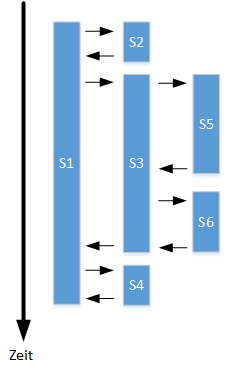
\includegraphics[width=0.5\textwidth]{Rayden-Scope.png}
\caption{Gültigkeitsbereiche in einem Rayden-Test}
\label{fig:rayden-scope}
\end{figure}

\SuperPar
In Rayden gibt es aber noch eine Besonderheit in Bezug auf Gültigkeitsbereiche. Rayden verwendet für die Gültigkeitsbereiche das Konzept von \enword{Dynamic Scoping}. Bei einem Aufruf eines \enword{Keywords} wird der Gültigkeitsbereich mit den Parametern angelegt. Das Besondere ist, dass der neue Gültigkeitsbereich eine Referenz auf den alten Gültigkeitsbereich hat. Das Resultat ist, dass jeder Kind-Gültigkeitsbereich Zugriff auf den Eltern-Gültigkeitsbereich hat.

\SuperPar
Ein Beispiel dazu sieht man in der Abbildung \ref{fig:rayden-scope}. Beim Starten eines Tests wird der Gültigkeitsbereich G1 angelegt. Auf diesen Gültigkeitsbereich haben später alle anderen Gültigkeitsbereiche Zugriff. Daher eignet sich dieser Gültigkeitsbereich gut für globale Variablen.

\SuperPar
In der Abbildung sieht man weiter, dass jeder neue Gültigkeitsbereich eine Beziehung zu einem Eltern-Gültigkeitsbereich hat. Der Pfeil von einem Kind- zu einem Eltern-Gültigkeitsbereich mag am Anfang komisch wirken. Den Pfeil kann man aber damit erklären, dass es in Rayden möglich ist, einen \enword{Out-} bzw. \enword{InOut}-Parameter zu definierten. Damit können Variablen aus G2 an G1 übertragen werden. Eine detaillierte Beschreibung zu den Parametern findet man im Abschnitt \ref{cha:Parameter}.

\SuperPar
Der Vorteil von vererbten Gültigkeitsbereichen ist, dass nicht alle Variablen übergeben werden müssen, welche bei einem Test zahlreich vorkommen können. Die Parameter bieten die Möglichkeit, für eine explizite Definition von Variablen. Das wird verwendet, um sicherzustellen, dass eine Variable definitiv zur Verfügung steht bzw. erleichtert auch die Verwendung eines \enword{Keywords}.

%%------------------------------------------------------------------------------------------------------
%\subsection{Benennung}
%\todo 

%%------------------------------------------------------------------------------------------------------
\subsection{Parameter}
\label{cha:Parameter}

\enword{Keywords} unterstützen das Definieren von Parametern für eine einfachere Verwendung. Grundsätzlich werden Parameter in Rayden nicht zwingend benötigt, da Rayden das Konzept von vererbten Gültigkeitsbereichen verwendet. Parameter ermöglichen jedoch eine explizite Schnittstelle für \enword{Keywords}. 

\begin{program}
\begin{JavaCode}
keyword Parameter Bespiel {
	
	parameter in    parm1
	parameter in    parm2 as string
	parameter out   param3 as boolean
	parameter inout param4 as number
	
	Test1	
}
\end{JavaCode}
\caption{Verwendung von Parametern}
\label{prog:parameter}
\end{program}


\SuperPar
Rayden unterstützt sowohl typisierte als auch untypisierte Parameter. Sind die Parameter typisiert, werden diese vom Rayden-Interpreter überprüft. Sind keine Werte für einen Parameter vorhanden, wird die Ausführung mit einem Fehler abgebrochen. 

\SuperPar
Neben einem Typ kann man bei einem Parameter auch noch die Richtung definieren. Die Richtung bezieht sich auf die Gültigkeitsbereich. In Rayden werden die Richtungen \enword{In}, \enword{Out} und \enword{InOut} unterstützt, wie man im Code-Beispiel \ref{prog:parameter} sehen kann. \\

\begin{itemize}
\item \textbf{\enword{In}-Parameter}\\
Der \enword{In}-Parameter transferiert einen Wert aus dem Eltern-Gültigkeitsbereich in den Kinder-Gültigkeitsbereich. Das ist auch das Standardverhalten, falls keine Richtung bei einem Parameter definiert ist.\\

\item \textbf{\enword{Out}-Parameter}\\
Der \enword{Out}-Parameter ist das genaue Gegenteil zum \enword{In}-Parameter. Dabei wird ein Wert aus dem Kinder-Gültigkeitsbereich in den Eltern-Gültigkeitsbereich transferiert. \\

\item \textbf{\enword{InOut}-Parameter}\\
Der dritte Variante ist eine Kombination aus dem \enword{In}-Parameter und dem \enword{Out}-Parameter.\\
\end{itemize}

%%------------------------------------------------------------------------------------------------------
\section{Datentypen von Rayden}

Die Sprache Rayden unterstützt die folgenden Datentypen:

\begin{itemize}
\item \enword{number},
\item \enword{string},
\item \enword{boolean},
\item \enword{variable},
\item \enword{location} und
\item \enword{enumeration}.
\end{itemize}

\SuperPar
Darunter befinden sich einige Standard-Datentypen wie \enword{number}, \enword{string} und \enword{boolean}. 

\begin{program}
\begin{JavaCode}
keyword Open Browser { 
	parameter in browserType as enumeration (IE | FF | CHROME)

	implemented in java -> "selenium.OpenBrowserKeyword"
}
\end{JavaCode}
\caption{Verwendung von einem \enword{enumeration}-Parameter}
\label{prog:enum}
\end{program}

\SuperPar
Der Typ \enword{enumeration} wird intern als \enword{string} repräsentiert. Die Laufzeitumgebung sorgt dafür, dass nur die vordefinierten Werte zugewiesen werden dürfen. Diese Überprüfung wird aber nur bei einem Übergang von einem Gültigkeitsbereich in einen anderen Gültigkeitsbereich vorgenommen. Diese Einschränkung ist damit zu erklären, dass ein \enword{enumeration}-Datentyp genau für ein \enword{Keyword} definiert wird. Ein Beispiel dazu sieht man im Code-Ausschnitt \ref{prog:enum}.  

\SuperPar
Ein weiterer spezieller Datentyp ist \enword{location}. Mit diesem Datentyp kann man ein Objekt in einem \enword{Object-Repository} referenzieren. Ein Wert dieses Datentyps beginnt immer mit einem @-Symbol. Nachfolgend kann man einen Pfad im \enword{Object-Repository} beschreiben, wie man im Beispiel \ref{prog:locator} sehen kann. Für Abnahme-Tests ist das Referenzieren von Test-Objekten essentiell. Daher bietet Rayden dafür eine Erleichterung. 

\begin{program}
\begin{JavaCode}
Click Left( @PetClinic.PetClinicWeb.Login.Go )
@PetClinic.PetClinicWeb.Login.Go :: Click Left
\end{JavaCode}
\caption{Verwendung vom Datentyp \enword{location}}
\label{prog:locator}
\end{program}

\SuperPar
Falls der erste Parameter von einem \enword{Keyword} vom Datentyp \enword{location} ist, kann man diesen Parameter vor das \enword{Keyword} schreiben. Somit wird das Lesen eines Tests erleichtert. Ein Verwendung dazu findet man ebenfalls im Beispiel \ref{prog:locator}. Dieses Sprachfeature wird von der Rayden-Laufzeitumgebung wieder in einen klassischen \enword{Keyword}-Aufruf umgebaut.

\begin{program}
\begin{JavaCode}

keyword For Keyword Beispiel{
	For (i, 0, 2){
		Print("Hello - " + i)
	}
}

keyword For { 
	parameter in var as variable
	parameter in from as number
	parameter in to as number

	implemented in java -> "com.github.thomasfischl.rayden.runtime.keywords.impl.ForKeyword"
}
\end{JavaCode}
\caption{Verwendung vom Datentyp \enword{variable}}
\label{prog:variable}
\end{program}

\SuperPar
Der letzte Datentyp ist \enword{variable}. Dieser Datentyp wird verwendet, wenn man den Namen einer Variable an ein \enword{Keyword} übergeben will. Dieser Datentyp beeinflusst die Auswertung von Ausdrücken. Wird ein Ausdruck mit dem Datentyp \enword{variable} typisiert, werden alle Verwendungen von Variablen in diesem Ausdruck nicht ausgewertet. Ein gutes Beispiel dazu ist das \enword{For-Keyword} aus dem Code-Ausschnitt \ref{prog:variable}.

\SuperPar
In diesem Beispiel ist der Parameter \enword{var} als \enword{variable} deklariert. Dadurch wird der Ausdruck \enword{i} nicht ausgewertet, sondern als Zeichenkette der \enword{Keyword}-Implementierung übergeben. Somit kann die Implementierung eine neue Variable mit dem Namen \enword{i} anlegen. Würde man den Parameter \enword{var} mit einem anderen Datentyp versehen, würde die Ausführungseinheit für Ausdrücke versuchen, diese Variable mit einem Wert aus dem Gültigkeitsbereich zu ersetzen. Wird kein Wert für \enword{} gefunden, wird die Ausführung mit einem Fehler abgebrochen.

\SuperPar
Eine Typumwandlung ist in der Sprache Rayden nicht vorgesehen. Es ist zwar möglich, dass man alle Datentypen zu einem \enword{string}-Datentyp umwandeln kann, aber alle anderen Kombinationen sind nicht möglich. In der Implementierung von einem \enword{Keyword} können die Werte beliebig konvertiert werden. Die Laufzeitumgebung stellt den Datentyp nur innerhalb der Gültigkeitsbereiche sicher.

%%------------------------------------------------------------------------------------------------------
\section{Verarbeiten von \enword{Keywords} und Ausdrücken}

Im Rayden-System ist der Interpreter und die \enword{Runtime} für die Ausführung eines Tests zuständig. Dabei wird die Ausführung von \enword{Keywords} und Ausdrücken von einander getrennt. Die \enword{Keywords} werden von einer \enword{Stack}-Maschine ausgeführt. 

\SuperPar
Die Ausdrücke werden in einer eigenen Ausführungseinheit behandelt. Die Ausführungseinheit verwendet keine \enword{Stack}-Maschine, sondern den rekursiven Abstieg für die Auswertung. Dabei kann diese Einheit entweder untypisiert oder typisiert ausgeführt werden. Diese Eigenschaft zur Typisierung von Parametern wird benötigt, um die Funktionalität einiger Datentypen zu ermöglichen. Darunter fallen die Datentypen \enword{variable} und \enword{enumeration}. Für diese beiden Datentypen muss sich die Ausführungseinheit entweder anders verhalten oder zusätzliche Überprüfungen durchführen. 

%%------------------------------------------------------------------------------------------------------
\section{\enword{Library} und \enword{Bridge}}

Um mit Rayden auch große Testprojekte verwalten zu können, gibt es das Konzept von Bibliotheken (\enword{Libraries}). Eine Bibliothek besteht aus einer Menge von \enword{Keywords}. Es können sowohl \enword{Scripted-}, \enword{Scripted-Compound-} also auch \enword{Compound-Keywords} in einer Bibliothek enthalten sein. Wobei man wahrscheinlich eher \enword{Scripted-} und \enword{Scripted-Compound-Keywords} in einer typischen Bibliothek finden wird.  

\begin{program}
\begin{JavaCode}
keyword For { 
	parameter in var as variable
	parameter in from as number
	parameter in to as number

	implemented in java -> "com.github.thomasfischl.rayden.runtime.keywords.impl.ForKeyword"
}

keyword If { 
	parameter in condition as boolean

	implemented in java -> "com.github.thomasfischl.rayden.runtime.keywords.impl.IfKeyword"
}

keyword Print {
	parameter text
	implemented in java ->"com.github.thomasfischl.rayden.runtime.keywords.impl.PrintKeyword"
}
\end{JavaCode}
\caption{Bibliothek: \enword{stdlibrary.rlg}}
\label{prog:library}
\end{program}

\SuperPar
In einer Bibliothek werden \enword{Keywords} thematisch zusammengefasst. Man kann sich zum Beispiel vorstellen, dass es eine Standard-Bibliothek gibt, wie im Code-Beispiel \ref{prog:library} zu sehen ist. In diesem Beispiel sind \enword{For-, If-} und \enword{Print-Keyword}-Definitionen enthalten. Die Datei \enword{stdlibrary.rlg} und das dazugehörige \enword{Java}-Archiv bilden eine Rayden-Bibliothek. 

\SuperPar
Um eine Bibliothek verwenden zu können, muss man diese über eine \enword{import library} Direktive einbinden. Ein Beispiel sieht man dazu im Code-Ausschnitt \ref{prog:libraryUsage}. Nachdem die Bibliothek eingebunden wurde, können alle \enword{Keywords} daraus verwendet werden. Für \enword{Keywords} gibt es nur einen Namensraum. Falls es durch das Einbinden von Bibliotheken zu Namenskonflikten kommen sollte, wird die erste Implementierung, die gefunden wird, verwendet. In der Reihenfolge kommen zuerst die aktuellen \enword{Keywords} aus der Datei und danach die Bibliotheken in der Reihenfolge, in welcher diese definiert wurden.

\begin{program}
\begin{JavaCode}
import library "stdlibrary"

keyword Library Beispiel {
	If (1 == 1){
		Print("Condition is true")
	}
	For ("i", 0, 2){
		Print("Hello - " + i)
	}
}
\end{JavaCode}
\caption{Verwendung der \enword{StdLib} Bibliothek}
\label{prog:libraryUsage}
\end{program}

\SuperPar
In Rayden wird zwischen einer \enword{Library} und einer \enword{Bridge} unterschieden. In dieser Ausbaustufe des Rayden-Systems ist die Unterscheidung jedoch nur semantisch. 

\SuperPar
Unter einer \enword{Library} versteht man grundlegende Funktionen wie Schleifen, Verzweigungen und Validierungen. Im Gegensatz dazu besteht eine \enword{Bridge} aus \enword{Keywords}, welche spezifisch für eine Anwendungstechnologie sind. Dazu ist eine \enword{Bridge} auch meistens mit einem Testtreiber gekoppelt, welcher die Basisfunktionen zur Verfügung stellt. Die \enword{Keywords} kapseln die Funktionalität aus dem Testtreiber und stellen diese zur Verfügung. Eine \enword{Bridge} kann zum Beispiel das Steuern eines Browsers unterstützen und verwendet dazu Selenium. 


%%------------------------------------------------------------------------------------------------------
\section{\enword{Object Repository}}

Das \enword{Object Repository} stellt eine Abstraktion zur Test-Anwendung her. Alle Test-Objekte, welche in einem Test verwendet werden, können in einem \enword{Object Repository} verwaltet werden. In den Tests muss nicht jedes Mal der volle Bezeichner für das Test-Objekt verwendet werden, sondern nur eine Referenz darauf. 

\begin{program}
\begin{JavaCode}

objectrepository PetClinic {

	application PetClinicWeb {
		location absolute "/browser"
		
		page Login {
			location "/body/div/div[text='bla']"
			
			button Go {
				location "/btn[text='GO']"
			}
			
			control<Special Button> Cancel {
				location "/div[text='Cancel']"
			}
		
			textfield Username {
				location  "/input[id='username']"
			}
			
			textfield Password {
				location  "/input[id='password']"
			}			
		} 
	}
}
\end{JavaCode}
\caption{\enword{Object-Repository}}
\label{prog:or}
\end{program}

\SuperPar
Die Test-Objekte werden im \enword{Object Repository} in einem Baum verwaltet und können über diesen auch referenziert werden. Das Beispiel \ref{prog:or} zeigt ein \enword{Object Repository} für eine Webanwendung, welche als Bezeichner einen \enword{XPath}-Ausdruck verwendet.  Der Vorteil davon ist, das der Bezeichner \enword{location} über die Baumstruktur zusammengebaut wird. Dadurch erspart man sich viel Wartungsaufwand. 

\SuperPar
Typischerweise werden in einem \enword{Object Repository} nur Test-Objekte von einer Test-Anwendung zusammengefasst. Werden in einem Test mehrere Anwendungen getestet, sollten dafür unterschiedliche \enword{Object Repositories} angelegt werden.

\begin{program}
\begin{JavaCode}
page Main Page{
	list Owners (index) {
		location  "/ul/ur[$index]"
	}
}

\end{JavaCode}
\caption{\enword{Parametrisiertes Test-Objekt}}
\label{prog:orParam}
\end{program}

\SuperPar
Es ist auch möglich, das man ein Test-Objekt in einem \enword{Object Repository} parametrisiert. Damit können zum Beispiel Listen abgebildet werden, indem der Index als Parameter definiert wird. Ein Beispiel dazu findet man im Code-Ausschnitt \ref{prog:orParam}. Im Bezeichner \enword{location} werden keine Ausdrücke unterstützt. Die Parameter werden über eine Substituierung ersetzt und benötigen daher keinen Datentyp.


%% UI Control Coverage 
%% Ableiten von neuen Tests

%%------------------------------------------------------------------------------------------------------
\section{\enword{Java-Scripting-API}}

Das Rayden-System implementiert das\enword{Java-Scripting-API}. Durch diese Implementierung kann man in jedem \enword{Java}-Programm einen Rayden-Test ausführen. Somit lässt sich das Rayden-System in viele unterschiedliche Szenarien einbinden. 

\begin{program}
\begin{JavaCode}
ScriptEngineManager manager = new ScriptEngineManager();
manager.registerEngineName("RaydenLangScriptEngine", new RaydenScriptEngineFactory());
\end{JavaCode}
\caption{Code-Beispiel: \enword{ScriptEngineFactory} für Rayden registrieren}
\label{prog:registerFactory}
\end{program}

\SuperPar
Um einen Rayden-Test in ein \enword{Java}-Programm einbinden zu können, muss man zuerst die \enword{RaydenScriptEngineFactory} registrieren. Damit gibt man dem \enword{ScriptEngineManager} eine neue Sprache bekannt. Im Code-Beispiel \ref{prog:registerFactory} sieht man eine Möglichkeit, wie man die Rayden-Sprache über einen Namen registrieren kann. Es gibt auch noch andere Möglichkeiten, wie etwa das Registrieren über die Dateiendung.

\begin{program}
\begin{JavaCode}
ScriptEngineManager manager = new ScriptEngineManager();
ScriptEngine engine = manager.getEngineByName("RaydenLangScriptEngine");
Object result =  engine.eval(new FileReader("./test/simple-test.rlg"));
RaydenScriptResult resultObj = (RaydenScriptResult) result;
\end{JavaCode}
\caption{Code-Beispiel: Ausführen eines Rayden-Tests}
\label{prog:runEngine}
\end{program}

\SuperPar
Über die \enword{ScriptEngineFactory} kann der \enword{ScriptEngineManager} eine neue Instanz einer \enword{ScriptEngine} anlegen. Das Code-Beispiel \ref{prog:runEngine} zeigt, wie man einen Test aus einer Datei einliest und diesen über die \enword{ScriptEngine} ausführen lassen kann.

\SuperPar
In diesem Kapitel wurde der Aufbau und die Verwendung des Rayden-Systems beschrieben. Im nächsten Kapitel wird ein Testprojekt mit dem Rayden-System umgesetzt. Dazu werden alle vorher beschriebenen Testmethoden angewendet.


\chapter{Implementierung von Rayden}
\label{cha:Implementierung}

Diese Kapitel beschreibt die Implementierung von ausgewählten Komponenten des Rayden-System. Der Abschnitt \ref{cha:KeywordGrammar} zeigt die Grammatik und die \enword{Stack}-Maschine für die Ausführung von \enword{Keywords}. Es wird auf einzelne Implementierungsdetails detailliert eingegangen.  

\SuperPar
Im zweiten Abschnitt \ref{cha:Eval} wird der Aufbau von Ausdrücken beschrieben. Beendet wird dieser Abschnitt mit einem Auszug aus der \enword{RaydenExpressionEvaluator} Klasse, welche für die Auswertung der Ausdrücke zuständig ist. 

\SuperPar
Danach wird in Abschnitt \ref{cha:validateKeyword} die Validierung von Rayden-Tests gezeigt. Dafür wird das Validierungssystem von \enword{xText verwendet}. Abgeschlossen wird diese Kapitel mit dem Abschnitt \ref{cha:implementJSA}, welcher zeigt, wie die Integration des Rayden-Systems in das \enword{Java-Scripting-API} umgesetzt worden ist. 

%%------------------------------------------------------------------------------------------------------

\section{Umsetzung der \enword{Keyword}-Grammatik}
\label{cha:KeywordGrammar}

Die Rayden-Sprache wurde mit dem xText \cite{xtext} Compilerwerkzeug umgesetzt. Die Abbildung \ref{fig:keywordGrammar} zeigt einen Auszug aus der Grammatik für die Rayden-Sprache. Der Auszug zeigt die Grammatikregeln für \enword{Keywords}. Die Regel \enword{KeywordDecl} beginnt die Definition eines neuen \enword{Keywords}. Am Beginn der Regel wird der Typ für das \enword{Keyword} definiert. Eine Beschreibung und Auflistung der Typen ist in Abschnitt \ref{cha:KeywordTypes} enthalten. Danach folgt ein Name für das \enword{Keyword} welcher von einer öffneten geschwungenen Klammer gefolgt wird.

\begin{figure}
\centering
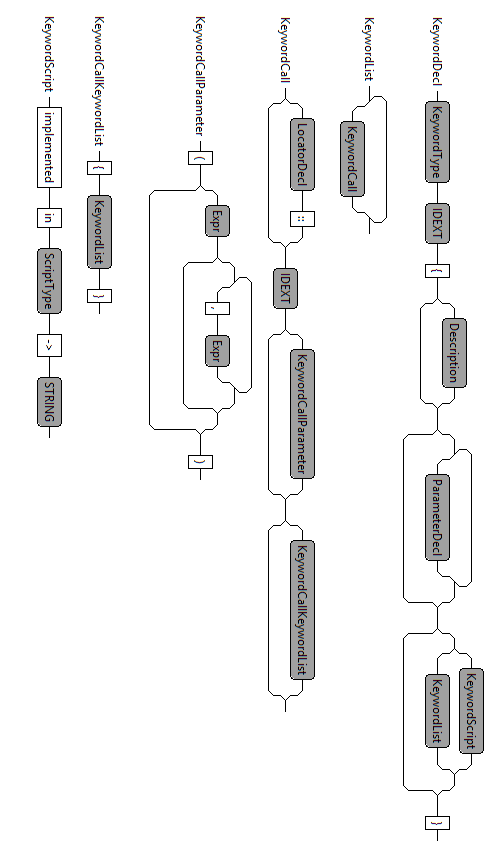
\includegraphics[width=0.9\textwidth]{grammar-keyword-all.png}
\caption{Auszug aus der Grammatik für \enword{Keywords}}
\label{fig:keywordGrammar}
\end{figure}

\SuperPar
Die geschwungenen Klammer definieren den Bereich der \enword{Keyword}-Implementierung. Am Anfang der Implementierung kann eine optionale Beschreibung angeführt werden. Diese wird von einer Parameterliste gefolgt. Ein Parameter wird mit der Regel \enword{ParameterDecl} beschrieben und kann 0 bis N Mal wiederholt werden. Eine Parameter-Definition besteht aus dem Schlüsselwort \enword{parameter}, einen Namen, einen Datentyp und einer Richtung.

\SuperPar
Danach folgt entweder die Bindung an ein Codestück mit der Regel \enword{KeywordScript} oder die \enword{Keyword}-Liste mit der Regel \enword{KeywordList} im Fall eines \enword{Compound-Keywords}. Die beiden Regeln sind wiederum optional um \enword{Keyword}-Rümpfe anlegen zu können. Diese Eigenschaft ist hilfreich, wenn die Testmanagerin oder der Testmanager nur die Struktur festlegen möchte, die Umsetzung des \enword{Keywords} jedoch von einem anderen Testpersonal vorgenommen wird. 

\begin{program}
\begin{JavaCode}
  Type Text (@PetClinic.PetClinicWeb.Login.Username , "max.mustermann")
	@PetClinic.PetClinicWeb.Login.Username :: Type Text ("max.mustermann")
	
	
	Click Left( @PetClinic.PetClinicWeb.Login.Go )
  @PetClinic.PetClinicWeb.Login.Go :: Click Left
\end{JavaCode}
\caption{Syntaktischer Zucker für die Verwendung von \enword{location}-Datentypen}
\label{prog:locatorSugar}
\end{program}

\SuperPar
Die Regel \enword{KeywordCall} definiert den Aufruf von einem \enword{Keyword} in einer \enword{Keyword}-Liste. Die Regel fängt normalerweise mit dem Namen des aufzurufenden \enword{Keywords} an. Danach folgt optional die Parameterliste für den Aufruf von dem \enword{Keyword}. Die Regel \enword{KeywrodCallParameter} definiert die Parameterliste, welche durch runde Klammer umschlossen ist. Die Parameter können als Liste von \enword{Expr}-Regeln definiert werden und werden durch einen Beistrich separiert werden. Für die einfachere Verwendung und besserer Lesbarkeit enthält die Regel \enword{KeywordCall} auch noch syntaktischen Zucker. Falls der erste Parameter von einem \enword{Keyword} vom Typen \enword{location} ist, kann diese Parameter vor das \enword{Keyword} geschrieben werden. Somit lässt sich die Implementierung leicht lesen. Der Codeausschnitt in Abbildung \ref{prog:locatorSugar} zeigt dazu die Verwendung des syntaktischen Zuckers im Vergleich zur klassischen Verwendung. Am Ende der \enword{KeywordCall}-Regel ist es noch möglich eine \enword{Keyword}-Liste zu definieren. Diese wird benötigt, falls es sich um ein \enword{Scripted-Compound-Keyword} oder um ein \enword{Inline-Keyword} handelt.

%%------------------------------------------------------------------------------------------------------

\section{Ausführung von \enword{Keywords} mit einer \enword{Stack}-Maschine}
\label{cha:StackMachine}

Im vorigen Abschnitt \ref{cha:KeywordGrammar} wurde die Grammatik von einem \enword{Keyword} in der Sprache Rayden erklärt. Dieser Abschnitt beschäftigt sich mit der Ausführung von \enword{Keywords}. Damit die \enword{Stack}-Maschine arbeiten kann, benötigt diese einen Zugriff auf den abstrakten Syntaxbaum. 

\begin{figure}
\centering
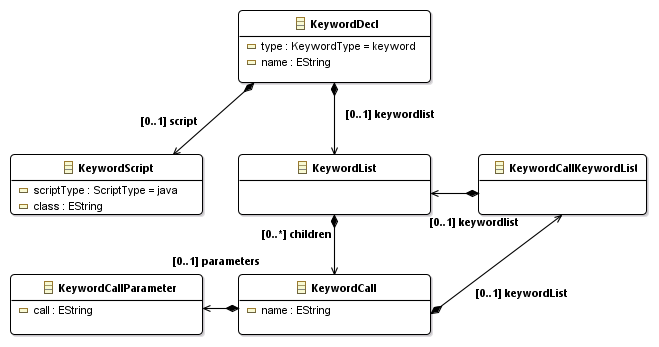
\includegraphics[width=1\textwidth]{keyword-model-diagramm.png}
\caption{Ausschnitt aus dem Abstrakte Syntaxbaum}
\label{fig:AST}
\end{figure}

\SuperPar
Das Compilerwerkzeug \enword{xText} stellt dafür ein \enword{Eclispe-ECore}-Modell zur Verfügung. Der generierten Compiler ist so konzipiert, dass dieser die gesamte Datei einliest und daraus einen abstrakten Syntaxbaum generiert. Der Syntaxbaum steht für die weitere Verarbeitung als \enword{ECore}-Modell zur Verfügung. Einen Auszug aus dem Modell zeigt die Abbildung \ref{fig:AST}. Die Abbildung zeigt die Modell-Repräsentation der Grammatik-Regeln von Abbildung \ref{fig:keywordGrammar}. Dieser Ausschnitt aus dem Modell stellt die Basis für die \enword{Stack}-Maschine dar. 

\SuperPar
Die \enword{Stack}-Maschine für das Rayden-System ist in der Klasse \enword{RaydenRuntime} implementiert. Der Codeauszug \ref{prog:runtime} zeigt die essentielle Methode \enword{executeKeyword}, welche für die Ausführung verantwortlich ist. Die Methode wird mit einem \enword{KeywordCall}-Objekt aufgerufen. Diese Objekt bezeichnet das erste \enword{Keyword}, welches von der \enword{Stack}-Maschine aufgerufen wird. Als erstes wird in der Methode übriggebliebene Element von dem \enword{Stack} entfernt. Danach wird über das \enword{Reporter-Interface} alle Objekte notifiziert, dass ein neuer Testfall gestartet worden ist. Im nächsten Schritt wird ein neuer Gültigkeitsbereich (\enword{RaydenScriptScope}) angelegt und mit dem \enword{KeywordCall}-Objekt initialisiert. Der Gültigkeitsbereich wird dann auf den leeren \enword{Stack} geladen. 

\SuperPar
Nach der Initialisierung der \enword{Stack}-Maschine wird die Abarbeitung gestartet. Es werden nun solange die Gültigkeitsbereiche am \enword{Stack} abgearbeitet, bis der \enword{Stack} leer ist oder ein Fehler bei der Ausführung von einem \enword{Keyword} aufgetreten ist. Der Gültigkeitsbereich repräsentiert einen Aufruf von einem \enword{Keyword} und die dazugehörigen Parameter und Variablen. Der Gültigkeitsbereich speichert zusätzlich die aktuelle Position in der \enword{Keyword}-Liste, falls es sich um ein \enword{Compound-Keyword} oder \enword{Scripted-Compound-Keyword} handelt. Über die Methode \enword{getNextOpt} kann die \enword{Stack}-Maschine das nächste \enword{Keyword} aus dem aktuellen Gültigkeitsbereich laden. Liefert die Methode kein Wert, ist die Ausführung des Gültigkeitsbereiches am Ende und wird daher vom \enword{Stack} entfernt.

\begin{program}
\lstinputlisting{samplecode/Runtime.java}
\caption{Codeauszug aus der \enword{RaydenRuntime}-Klasse}
\label{prog:runtime}
\end{program}

\SuperPar
Wurde jedoch ein Wert zurückgeliefert, wird mit der Ausführung fortgefahren. Handelt es sich bei dem Wert um ein \enword{KeywordCall}-Objekt, wird die Methode \enword{executeKeywordCall} aufgerufen. Diese Methode löst den Aufruf des \enword{Keywords} über eine \enword{Lookup}-Tabelle auf. Wurde die passende \enword{Keyword}-Implementierung gefunden, wird ein neuer Gültigkeitsbereich angelegt und auf den \enword{Stack} geladen. Wird in der \enword{Lookup}-Tabelle keine passende Implementierung gefunden, wird ein Fehler geworfen und die Ausführung abgebrochen. Handelt es sich jedoch um ein \enword{KeywordDecl}-Objekt wird das \enword{Keyword} ausgeführt.  

\SuperPar
Dabei muss die \enword{Stack}-Maschine überprüfen, ob es sich um ein \enword{Scripted-Compound-Keyword} handelt. Bei einem \enword{Scripted-Compound-Keyword} muss eine andere Logik ausgeführt werden, da es sowohl eine Code-Implementierung als auch eine \enword{Keyword}-Liste vorhanden ist. Bei allen anderen \enword{Keyword}-Metatypen wird die Methode \enword{executeKeywordDecl} ausgeführt. Diese Methode führt bei einem \enword{Scripted-Keyword} das spezifizierten Codestück aus. Bei einem \enword{Compound-Keyword} wird die \enword{Keyword}-Liste in den Gültigkeitsbereich geladen.

\SuperPar
Wurden alle Gültigkeitsbereich am \enword{Stack} erfolgreich abgearbeitet wird am Ende noch das \enword{Reporter-Interface} aufgerufen. Danach wird die Ausführung der \enword{Stack}-Maschine beendet.

%%------------------------------------------------------------------------------------------------------
\clearpage

\section{Auswertung von Ausdrücken}
\label{cha:Eval}

Dieser Abschnitt befasst sich mit den Grammatik-Regeln und der Ausführung von Ausdrücken. Die Rayden-Sprache unterstützt in einigen Bereichen der Sprache Ausdrücke. Ein Ausdruck kann in der Grammatik mit der Regel \enword{Expr} aufgerufen werden. Die Abbidlung \ref{fig:exprGrammar} zeigt einen Überblick über die Grammatik-Regeln von Ausdrücke. 

\begin{figure}
\centering
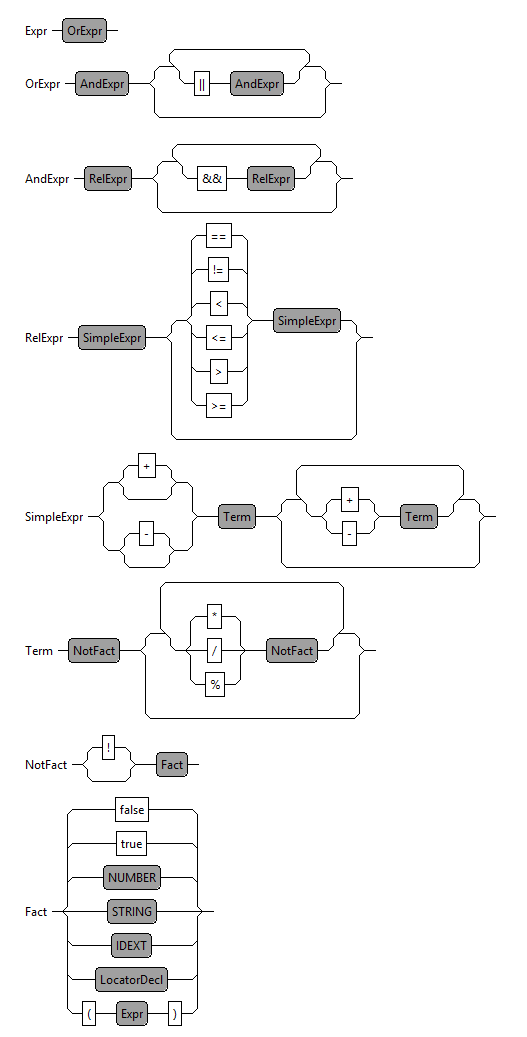
\includegraphics[width=0.9\textwidth]{grammar-expr.png}
\caption{Grammatik-Regeln für Ausdrücke}
\label{fig:exprGrammar}
\end{figure}

\SuperPar
Die Regeln für den Ausdruck sind klassisch aufgebaut. Die Operationen sind nach der Ausführungsreihenfolge in den Regeln eingearbeitet. Die am stärksten bindenden Operationen befinden sich in der Nähe der Blätter des Ausdrucksbaum. Die schwach bindenden Operationen befinden sich in der Nähe des Wurzelknotens. Die Blätter repräsentieren die Werte in einem Ausdruck, welche in der Regel \enword{Fact} definiert werden. Die Werte können entweder Konstanten oder Variablen sein und haben eine definierten Datentypen. Die Regel \enword{Fact} hat jedoch keinen spezielle Behandlung für \enword{Enumerations}. Der Grund dafür ist, dass \enword{Enumerations} intern als \enword{Strings} verarbeitet werden. Die Validierung der\enword{Enumerations} wird nur beim Initialisieren von Gültigkeitsbereichen durchgeführt.

\SuperPar
Für die Ausführung von Ausdrücken ist im Rayden-System die Klasse \enword{RaydenExpressionEvaluator} zuständig. Der Codeausschnitt \ref{prog:evaluator} zeigt eine Überblick über die Klasse \enword{RaydenExpressionEvaluator}. Die Klasse wird mit einem Gültigkeitsbereich initialisiert. Der Gültigkeitsbereich wird benötigt um Variablen bei der Abarbeitung auswerten zu können. 

\SuperPar
Die Auswertung eines Ausdrucks wird mit der Methode \enword{eval(Expr expression, String resultType)} gestartet. Als Parameter für die Methode wird ein \enword{Expr}-Objekt und eine Zeichenkette übergeben. Das \enword{Expr}-Objekt ist das Wurzelobjekt im \enword{ECore}-Modell für eine Ausdruck. Mit dem zweiten Parameter kann man die Auswertung des Ausdrucks typisieren. Wurde ein Typ definiert, wird am Ende der Auswertung noch überprüft, ob das Ergebnis vom selben Typ ist. Stimmt der Wert nicht überein, wird eine Fehler geworfen. Es gibt auch noch eine Spezialfall bei der Typisierung. Wird ein Ausdruck mit dem Typ \enword{variable} parametrisiert, werden keine Variablen im Ausdruck ausgewertet. Diese Eigenschaft wird benötigt, um Variablennamen an ein \enword{Keyword} übergeben zu können.

\SuperPar
Der Codeausschnitt \ref{prog:evaluator} enthählt am Ende die Implementierung der \enword{eval}-Methode für das Objekt \enword{Fact}. Diese Methode zeigt, wie die Werte aus dem \enword{ECore}-Modell nach \enword{Java} konvertiert werden. Die Methode zeigt auch, wie Variablen mithilfe des Gültigkeitsbereichs ausgewertet werden können.

\begin{program}
\lstinputlisting{samplecode/RaydenExpressionEvaluator.java}
\caption{Codeauszug aus dem \enword{RaydenExpressionEvaluator}}
\label{prog:evaluator}
\end{program}

%%------------------------------------------------------------------------------------------------------
\clearpage
\section{Überprüfung der \enword{Keyword}-Referenzen}
\label{cha:validateKeyword}

\begin{program}
\lstinputlisting{samplecode/Validator.java}
\caption{Codeauszug aus dem \enword{RaydenDSLJavaValidator}}
\label{prog:validator}
\end{program}

%%------------------------------------------------------------------------------------------------------

\section{Implementierung der \enword{Java-Scripting-API}}
\label{cha:implementJSA}

\begin{program}
\lstinputlisting{samplecode/ScriptEngine.java}
\caption{Codeauszug aus der \enword{RaydenScriptEngine}}
\label{prog:scriptEngine}
\end{program}

\todo


\chapter{Umsetzung eines Testprojektes mit Rayden}
\label{cha:Testen}

Es wird gezeigt, wie man ein Testprojekt mithilfe von Rayden umsetzten kann. Dabei wird eine einfache Webanwendung getestet. Zum Beispiel ein Rechner oder kleine Task Anwendung. Dafür werden alle Ebenen von funktionalen Tests durchgeführt.

%%------------------------------------------------------------------------------------------------------

\section{Beispielanwendung}

Für das Evaluieren des Rayden-Systems wird eine Anwendung zum Test benötigt. Bei der Anwendung sollte es sich um eine Webanwendung handeln, um die Unterstützung von Selenium zeigen zu können. Für die Evaluierung hat man sich für die \enword{PetClinic}-Webanwendung entschieden, welche eine Beispielanwendung des Spring-Projekts ist. Die Anwendung mit allen Ressourcen ist öffentlich auf Github unter der Adresse \enword{https://github.com/spring-projects/spring-petclinic/} zugänglich.

\begin{figure}
\centering
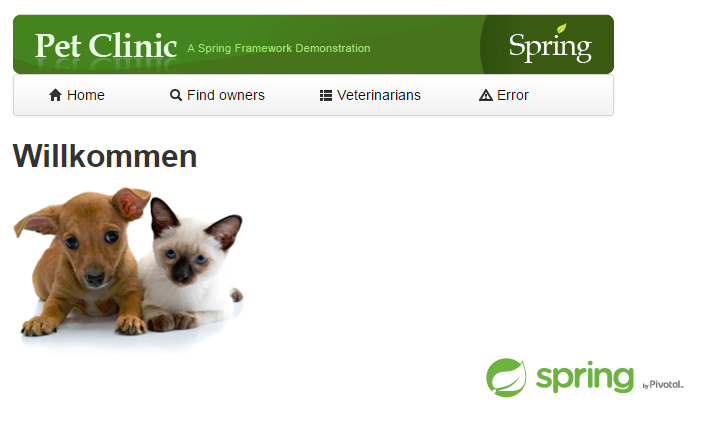
\includegraphics[width=0.9\textwidth]{petclinic.png}
\caption{Startseite der Webanwendung PetClinic}
\label{fig:petClinicPage}
\end{figure}

\SuperPar
Bei der \enword{PetClinic}-Anwendung handelt es sich um eine Verwaltungssoftware für eine Tierklinik. Mit der Anwendung können Besuche bei einem Tierarzt protokolliert werden. Dazu gehört die Erfassung der Tierbesitzer mit ihren Haustieren. Zu jedem Haustier werden alle Arztbesuche gespeichert, damit der Krankheitsverlauf dokumentiert ist. Neben den Besitzer und ihren Tieren werden Tierärztinnen und Tierärzte verwaltet. 

\SuperPar
Da der Funktionsumfang der Anwendung überschaubar ist, eignet sich diese ausgezeichnet als Beispielanwendung für die Evaluierung des Rayden-System. In den nächsten Abschnitten werden Test mit unterschiedlichen Testmethoden für die \enword{PetClinic}-Anwendung gezeigt.

\SuperPar
In den folgenden Abschnitte \ref{cha:TestenUnit}, \ref{cha:TestenApi} und \ref{cha:TestenUA} werden Tests für die \enword{Petclinic}-Anwendung vorgestellt. Diese Tests wurden mit drei unterschiedlichen Testmethoden umgesetzt um zu zeigen, wie man die Testmethoden mit dem Rayden-System vereinen kann.

%%------------------------------------------------------------------------------------------------------
\section{Komponententests}
\label{cha:TestenUnit}

Dieser Abschnitt zeigt die Umsetzung eines Komponententests mit dem Rayden-System. Für einen Komponententest wir in Rayden zuerst ein \enword{Keyword} angelegt. Der Codeauszug \ref{prog:unitTest} zeigt die Definition des \enword{Keywords}. Ein Komponententest wird normalerweise als \enword{Scripted-Keyword} umgesetzt und mit dem \enword{Keyword}-Typ \enword{unittest} gekennzeichnet. In diesem Beispiel wird die Komponente \enword{PetTypeFormatter} getestet. Die Komponente ist in der Webanwendung dafür verantwortlich, aus einer Zeichenkette das dazugehörige Domänenobjekt zu liefern und umgekehrt. 

\begin{program}
\begin{JavaCode}
unittest Test PetTypeFormatter {
	''' This unittest verifies the functionality of the 
	    formatter class PetTypeFormatter '''
	implemented in java -> "petclinic.TestPetTypeFormatterKeyword"
}
\end{JavaCode}
\caption{Komponententest \enword{Test PetTypeFormatter}}
\label{prog:unitTest}
\end{program}

\SuperPar
Der Codeausschnitt \ref{prog:unitTestImpl} zeigt die Implementierung des \enword{Scripted-Keywords}. Die Implementierung des Komponententests ist grundlegend gleich mit einem normalen \enword{JUnit}-Test. Die großen Unterschiede sind, dass die Methode nicht mit \enword{@Test} annotiert werden und dass es nur eine Testmethode pro Klasse geben kann. 

\begin{program}
\begin{JavaCode}
public class TestPetTypeFormatterKeyword implements ScriptedKeyword {

  @Override
  public KeywordResult execute(String keyword, KeywordScope scope, RaydenReporter reporter) {
    ClinicService service = new MockClinicService();
    PetTypeFormatter formatter = new PetTypeFormatter(service);

    try {
     Assert.assertEquals("dog", formatter.parse("dog", null).getName());
     Assert.assertEquals("cat", formatter.parse("cat", null).getName());
     Assert.assertEquals("fish",formatter.parse("fish",null).getName());
    } catch (ParseException e) {
      throw new AssertionError(e);
    }
    
    try {
      formatter.parse("hamster", null);
      Assert.fail("No ParseExeption was thrown!");
    } catch (ParseException e) {
    }

    try {
      formatter.parse(null, null);
      Assert.fail("No ParseExeption was thrown!");
    } catch (ParseException e) {
    }

    return new KeywordResult(true);
  }
}
\end{JavaCode}
\caption{Implementierung des \enword{Test PetTypeFormatter} \enword{Keywords}}
\label{prog:unitTestImpl}
\end{program}

\SuperPar
Eine nützliche Erweiterung des Rayden-Systems in der Zukunft wäre eine bessere Integration mit \enword{Unittest-Frameworks} wie \enword{JUnit} oder \enword{TestNG}.

%%------------------------------------------------------------------------------------------------------
\section{Schnittstellentest}
\label{cha:TestenApi}

Bei einem Schnittstellentest werden öffentliche Schnittstellen wie ein \enword{Restful}-Schnittstelle \cite{Rest} getestet. Im Schnittstellentest \ref{prog:integrationTest} wird die \enword{Restful}-Schnittstelle für Tierärzte getestet. Schnittstellentests können entweder als \enword{Compound-Keywords} oder als \enword{Scripted-Keywords} definiert werden. Es hängt ganz davon ab, ob die Implementierung des \enword{Scripted-Keywords} in einem anderen Test wieder verwendet werden kann. 

\begin{program}
\begin{JavaCode}
apitest Test Veterinarians Restful Service {
	'''This keyword checks the restfull service for veterinarian.'''
	
	Verify Json("http://localhost:9966/petclinic/vets.json", 
	            "./demodata/vets.json")
}

keyword Verify Json {
  '''The keyword download the content from the given url. A second 
	   content is loaded from the file. The both contents are parsed
		 into a JSON object tree. If the two trees were equals, the 
		 keyword finish successfully'''
		
	parameter url
	parameter file

	implemented in java -> "petclinic.VerifyJsonKeyword"
}
\end{JavaCode}
\caption{Integrationstest \enword{Test Veterinarians Restful Service}}
\label{prog:integrationTest}
\end{program}

\SuperPar 
Bei diesen Beispiel liefert die Schnittstelle das Ergebnis als einen JSON-Text. Um zu Überprüfen ob die Schnittstelle korrekt funktioniert, wird dieser Text mit einem Text aus einer Demodaten-Datei verglichen. Damit der Test erfolgreich durchläuft, müssen die beiden Texte semantisch Gleich sein. Semantisch Gleich heißt bei einem JSON-Text, dass die enthaltenen Daten gleich sein müssen, aber nicht in welcher Reihenfolge diese serialisiert worden sind.

\begin{program}
\begin{JavaCode}
public class VerifyJsonKeyword implements ScriptedKeyword {
  @Override
  public KeywordResult execute(String keyword, KeywordScope scope, RaydenReporter reporter) {
    String url = scope.getVariableAsString("url");
    String file = scope.getVariableAsString("file");

    try {
      CloseableHttpClient client = HttpClientBuilder.create().build();
      CloseableHttpResponse response = client.execute(new HttpGet(url));
      if (response.getStatusLine().getStatusCode() != 200) {
        return new KeywordResult(false);
      }
      String json = IOUtils.toString(response.getEntity().getContent());

      JsonParser parser = new JsonParser();
      JsonElement o1 = parser.parse(json);
      JsonElement o2 = parser.parse(IOUtils.toString(new FileInputStream(file)));

      return new KeywordResult(o1.equals(o2));
    } catch (IOException e) {
      throw new RuntimeException(e);
    }
  }
}
\end{JavaCode}
\caption{Implementierung des \enword{Verify Json Keywords}}
\label{prog:integrationTestImpl}
\end{program}

\SuperPar
Wenn mehrere Schnittstellen dieser Art getestet werden, ist es sinnvoll, dass man die Funktionalität zum Abfragen und Vergleichen der Daten in ein separates \enword{Keyword} kapselt. Dadurch können andere Tests dieses \enword{Keyword} wiederverwenden. Die Implementierung des \enword{Verify Json Keywords} zeigt das Codebeispiel \ref{prog:integrationTestImpl}. Das Codestück zeigt, dass zuerst über einen \enword{HttpClient} der JSON-Text von einem Server abgefragt wird. Danach wird der JSON-Text mit einem \enword{Parser} in einem Objektbaum transformiert. Dafür wird eine \enword{Parser}-Implementierung aus der \enword{Google-Guava}-Bibliothek verwendet. Der selbe Prozess wird auch mit der Demodaten-Datei durchlaufen. Am Ende gibt es zwei Objektbäume für die JSON-Texte. Für den semantischen Vergleich der beiden Bäume kann die Methode \enword{equals()} der Klasse \enword{JsonElement} verwendet werden. Diese Klasse stammt wiederum aus der \enword{Google-Guava}-Bibliothek.

%%------------------------------------------------------------------------------------------------------
\section{Abnahmetests}
\label{cha:TestenUA}

In diesem Abschnitt wird die letzte Testmethode für die Evaluierung erläutert. Dabei handelt es sich um Abnahmetests, die wohl wichtigste Testmethode für das Rayden-System. Ein Großteil des Rayden-System ist primär für die Unterstützung dieser Testmethode entwickelt worden. Aus diesem Grund enthält dieser Abschnitt auch zwei Umsätzungen von Testmethoden mit Rayden. Als erstes wird der Testfall \enword{Suchen nach einen Tierbesitzer} \ref{cha:TestenUA1} umgesetzt. Bei diesem Testfall wird die Suche der \enword{Petclinic}-Anwendung getestet. Im zweiten Testfall \ref{cha:TestenUA2} wird das Anlegen eines neuen Tierbesitzers gezeigt. 

\SuperPar
Für das Steuern der Browser wurde für beide Abnahmetests die Selenium-Bibliothek verwendet. Aus diesem Grund wird im dritten Teil \ref{cha:TestenSelenium} dieses Abschnittes die Bindung zwischen dem Rayden-System und der Selenium-Bibliothek gezeigt. 

%%------------------------------------------------------------------------------------------------------

\subsection{Abnametest \enword{Suchen nach einen Tierbesitzer}}
\label{cha:TestenUA1}

Bei dem  Abnahmetest im Codeausschnitt \ref{prog:uatest-find} wird die Suchfunktion der \enword{Petclinic}-Anwendung getestet. Dafür wird der Testfall als erstes in zwei \enword{Compound-Keywords} \enword{Find a specific Pet Owner} und \enword{Check Owner Details} aufgeteilt. Neben den beiden \enword{Keywords} werden noch zwei weiter \enword{Keywords} \enword{Prepare Browser} und \enword{Cleanup Browser}  benötigt, welche für das Starten und Stop des Browsers zuständig sind. 

\begin{program}
\lstinputlisting{samplecode/uatest-findpetowner.rlg}
\caption{Abnametests: \enword{Suchen nach einen Tierbesitzer}}
\label{prog:uatest-find}
\end{program}


\begin{program}
\lstinputlisting{samplecode/or-findpetowner.rlg}
\caption{Codeauszug aus dem \enword{Object-Repository} für den Testfall \enword{Suchen nach einen Tierbesitzer}}
\label{prog:or-find}
\end{program}

\SuperPar
Das \enword{Keyword} \enword{Find a specific Pet Owner} führt die Suche nach einem Tierbesitzer mit dem Name \enword{Davis} aus. Dafür navigiert das \enword{Keyword} auf die Seite für Tierbesitzer und startet die Suche nach allen Besitzern. Danach werden auf der Ergenbisseite der Suche alle Besitzer aufgelistet, welche in der Anwendung vorhanden sind. Danach wird mithilfe der integrierten Suche nach dem Namen \enword{Davis} gesucht und die Detailseite des Tierbestitzers geöffnet. Wurde die Detailseite erfolgreich geöffnet ist das \enword{Keyword} am Ende. Die Validierung der Daten werden von dem nächsten \enword{Keyword} \enword{Check Owner Details} durchgeführt.

\SuperPar
Dem \enword{Keyword} \enword{Check Owner Details} werden die zu überpüfenden Daten als Parameter übergeben. Das \enword{Keyword} überprüft jedes Datum mit dem \enword{Scripted-Keyword} \enword{Verify Text}. Dem \enword{Scripted-Keyword} werden zwei Parameter übergeben. Der erste Parameter ist ein \enword{Locator}, welcher ein Element auf der Webseite definiert. Von diesem Element wird der Text abgefragt und mit dem zweiten Parameter verglichen. Der zweite Parameter ist eine Zeichenkette mit dem erwarteten Wert. Sind die Wert nicht gleich, wird der Test mit einem Fehler abgebrochen. 

\SuperPar
Damit in den \enword{Keywords} keine \enword{XPath}-Ausdrücke vorkommen müssen, wird ein \enword{Objekt-Repository} verwendet. Einen Auszug mit den wichtigisten Objekten für diesen Abnahmetest zeigt das Codebeispiel \ref{prog:or-find}. Das Codebeispiel enthält die Objekte für die Suchergebnisseite und die Detailseite für Tierbesitzerinnen und Tierbesitzer.

\todo OR - Bild mit Ergebnis Webseite hinzufügen

%%------------------------------------------------------------------------------------------------------

\subsection{Abnametest \enword{Anlegen eines neuen Tierbesitzer}}
\label{cha:TestenUA2}

Der zweite Abnahmetest testet den Anwendungsfall \enword{Anlegen eines neuen Tierbesitzer}. Diese Abnahmetest wird direkt im Abnahmetest-\enword{Keyword} ausspezifiziert. Als erstes wird wiederum die Testumgebung mit dem \enword{Keyword} {Preapre Browser} vorbereit. Im nächsten Schritt navigiert der Test auf die Tierbesitzerseite und klick auf die \enword{Add Owner} Schlatfläche. 

\begin{program}
\lstinputlisting{samplecode/uatest-createpetowner.rlg}
\caption{Codeauszug: \enword{Anlegen eines neuen Tierbesitzer}}
\label{prog:uatest-create}
\end{program}

\SuperPar
Danach werden alle benötigten Daten für eine neue Tierbesitzerin oder Tierbesitzer eingegeben. Dazu wird das \enword{Keyword} \enword{Type Text} verwendet. 

\begin{program}
\lstinputlisting{samplecode/or-createpetowner.rlg}
\caption{Codeauszug aus dem \enword{Object-Repository} für den Testfall \enword{Anlegen eines neuen Tierbesitzer}}
\label{prog:or-create}
\end{program}

\todo

\clearpage
%%------------------------------------------------------------------------------------------------------

\subsection{Selenium \enword{Keywords}}
\label{cha:TestenSelenium}

\begin{program}
\lstinputlisting{samplecode/selenium.rlg}
\caption{Codeauszug aus der Selenium \enword{Keyword}-Bibliothek}
\label{prog:selenium}
\end{program}


\begin{program}
\begin{JavaCode}
public class OpenBrowserKeyword implements ScriptedKeyword {

	@Override
	public KeywordResult execute(String keyword, KeywordScope scope, RaydenReporter reporter) {
		String browserType = scope.getVariableAsString("browserType");
		String url = scope.getVariableAsString("url");
		WebDriver driver = Selenium.getInstance().initializeDriver(browserType);
		driver.navigate().to(url);
		return new KeywordResult(true);
	}
}
\end{JavaCode}
\caption{Implementierung des \enword{Open Browser Keywords}}
\label{prog:openBrowserKeyword}
\end{program}


\begin{program}
\begin{JavaCode}
public class ClickKeyword implements ScriptedKeyword {

  @Override
  public KeywordResult execute(String keyword, KeywordScope scope, RaydenReporter reporter) {
    RaydenExpressionLocator locator = (RaydenExpressionLocator) scope.getVariable("locator");
    reporter.log("Click on '" + locator + "'");
    Selenium.getInstance().findElement(locator.getEvalLocator()).click();
    return new KeywordResult(true);
  }
}
\end{JavaCode}
\caption{Implementierung des \enword{Click Keywords}}
\label{prog:clickKeyword}
\end{program}



\begin{program}
\begin{JavaCode}
public class VerifyTextKeyword implements ScriptedKeyword {

  @Override
  public KeywordResult execute(String keyword, KeywordScope scope, RaydenReporter reporter) {
    RaydenExpressionLocator locator = (RaydenExpressionLocator) scope.getVariable("locator");
    String text = scope.getVariableAsString("text");
    WebElement element = Selenium.getInstance().findElement(locator.getEvalLocator());
    String elementText = element.getText();
    reporter.log("Verify Text: '" + text + "'='" + elementText + "'");
    return new KeywordResult(text.equals(elementText));
  }
}
\end{JavaCode}
\caption{Implementierung des \enword{Verify Text Keywords}}
\label{prog:verifyTextKeyword}
\end{program}

\todo

\clearpage

\section{Testdokumentation}

TODO !!!

\chapter{Zusammenfassung}
\label{cha:Zusammenfassung}

Diese Masterarbeit hat zum Ziel, die Erstellung und die Wartung von Tests im Allgemeinen und im speziellen die Abnahmetests zu vereinfachen. Ein weiteres Ziel ist es, die Zusammenarbeit von Fach-, Entwicklungs- und Testabteilungen zu erleichtern. Dafür wurde im Kapitel \ref{cha:StandDerTechnik} die gängigsten Testmethoden und Technologien vorgestellt, welche in der Softwareentwicklung eingesetzt werden. Im nächsten Kapitel \ref{cha:Konzept} wurde der Ablauf von einem Testprojekt skizziert. Dabei wurde darauf eingegangen, welche Personengruppe in einem Testprojekt involviert sind und welche Aufgaben diese übernehmen. 

\SuperPar
Das Kapitel \ref{cha:Design} hat sich mit dem Design von Rayden beschäftigt. Am Anfang des Kapitels wurden die Ziel von Rayden beschrieben. In den nächsten Abschnitten wurde die Sprache von Rayden detailliert erklärt und die Verwendung eines \enword{Object-Repositories} gezeigt. Die Implementierung ausgewählt der Komponenten wird in Kapitel \ref{cha:Implementierung} gezeigt. Es wurde gezeigt, wie die \enword{Stack}-Maschine implementiert worden ist, welche für die Ausführung von \enword{Keywords} verantwortlich ist. Ein weiterer interessanter Punkt der Implementierung war die Integration des Rayden-System in das \enword{Java-Scripting-API}. 

\SuperPar
Im Kapitel \ref{cha:Testen} wurde das Rayden-System mithilfe einer Beispielanwendung evaluiert. Es wurden Tests mit unterschiedlichen Testmethoden für die Beispielanwendung geschrieben. Dabei wurde gezeigt, welche Vorteile Rayden bei der Umsetzung von Abnahmetests hat.

\section{Ausblick auf weitere Arbeiten}

Im Zuge der Arbeit an der Masterarbeit wurde einige Bereiche identifiziert, welche zukünftig erweitert werden können.\\

\begin{itemize}
\item Implementierung eines grafischen Editors für Rayden-Tests:\\

Um die Verwendung des Rayden-Systems zu erleichtern, würde eine visuelle Repräsentation von Tests helfen. Dazu müsste ein grafischer Editor für die Rayden-Sprache entwickelt werden. Das Ziel dieses Editors ist es, neu \enword{Compound-Keywords} anzulegen und bestehende zu warten. Auch eine visuelle Darstellung der Ausführung eines Tests in dem Editor würde die Handhabung erleichtern.\\

\item \enword{Debugger} für Rayden:

Da Rayden eine eigene Ausführungseinheit besitzt, können keine bestehenden \enword{Debugger} verwendet werden, um einen Rayden-Test zu analysieren. Darum wäre die Implementierung eines eigenen \enword{Debuggers} für die Sprache vorteilhaft. Zusätzlich könnte dieser Erweiterungen erlauben, dass man einen Test Schritt für Schritt ausführt. Somit können Fehler schneller aufgespürt und behoben werden.\\

\item Integration weiterer Sprachen:

In der derzeitigen Ausführung von Rayden können \enword{Scripted-Keywords} und \enword{Scripted-Compound-Keywords} nur mit \enword{Java} implementiert werden. Als Erweiterung könnte man zusätzliche Sprachen unterstützen. Spezielle Skriptsprachen wie \enword{JavaScript}, \enword{Python} oder \enword{Ruby} würden sich eignen. Der Vorteil davon wäre, dass man sich die Kompilierungsphase für die \enword{Scripted-Keywords} sparen würden. \\

\item Integration mit Test-Bibliotheken:

Bei der Umsetzung von Komponententests hat sich gezeigt, dass man nicht so einfach bestehenden Komponententests wiederverwenden kann. Daher würde es helfen, wenn man nicht nur Klassen mit dem Interface \enword{ScriptedKeyword} als Implementierung für \enword{Scripted-Keywords} verwenden kann. Die Erweiterung könnte dafür sorgen, dass zum Beispiel bestehenden JUnit-Tests als Implementierung verwendet werden können. Es müsste ein Adapter erstellt werden, der die Verbindung zwischen Rayden und einem Test-\enword{Framework} wie JUnit herstellt. Diese Erweiterung würde die Akzeptanz von Entwicklerinnen und Entwicklern steigern, da diese weiterhin mit ihren gewohnten Werkzeugen arbeiten können. 

\end{itemize}

\section{Erfahrungen}

Meine größte und wichtigste Erfahrung bei dieser Masterarbeit war die Erkenntnis, dass das Designen einer Sprache ein höchst komplexer Prozess ist. Das Design der Rayden-Sprache war äußerst anspruchsvoll, da die Sprache wenig Ähnlichkeiten zu bestehenden Sprachen hat. Daher gab es für das Sprachdesign etliche Iterationen bis das finale Konzept fertig war.

\SuperPar
Das \enword{xText-Framework} war das wichtigste Werkzeug bei der Erstellung der Sprache und des gesamten Systems. Ich hatte schon gut Erfahrungen mit dem \enword{xText-Framework} während der Bachelorarbeit gemacht. Aus diesem Grund habe ich dieses Werkzeug auch für die Masterarbeit wiederverwendet. Jedoch habe ich die Erfahrung gemacht, dass ich mit der Komplexität und den Besonderheiten der Rayden-Sprache die Grenzen von \enword{xText-Framework} erreicht habe.

\section{Danksagung}

Zu Beginn möchte ich mich ganz herzlich bei meinem Betreuer Herrn FH-Prof. DI Dr. Heinz Dobler bedanken. Herr Dobler hat mich bereits bei der Bachelorarbeit betreut und ich war froh, dass er mich wieder bei der Masterarbeit betreut hat. Neben se 






\todo


%%%----------------------------------------------------------
%%%Anhang
\appendix
%%\include{anhang_a}	% Technische Ergänzungen
%%\include{anhang_b}	% Inhalt der CD-ROM/DVD
%%\include{anhang_c}	% Chronologische Liste der Änderungen
%%\include{anhang_d}	% Quelltext dieses Dokuments

%%%----------------------------------------------------------
\MakeBibliography
%%%----------------------------------------------------------

%%%Messbox zur Druckkontrolle
%%\chapter*{Messbox zur Druckkontrolle}



\begin{center}
{\Large --- Druckgröße kontrollieren! ---}

\bigskip

\Messbox{100}{50} % Angabe der Breite/Hoehe in mm

\bigskip

{\Large --- Diese Seite nach dem Druck entfernen! ---}

\end{center}



\end{document}
